\documentclass[11pt,a4paper]{article}
\usepackage[utf8]{inputenc}
\usepackage[french]{babel}
\usepackage[T1]{fontenc}

\usepackage{amsmath}
\usepackage{amsfonts}
\usepackage{amssymb}

\newcommand{\TitreMatiere}{Algorithmique et Structures de Données 1}
\newcommand{\TitreSeance}{Listes, Piles, Files}
\newcommand{\NumeroTD}{Structures \& Pointeurs}
\newcommand{\DateCours}{Octobre 2022}
\newcommand{\AnneeScolaire}{2022-2023}
\newcommand{\Organisation}{EPITA}
\newcommand{\NomAuteurA}{Fabrice BOISSIER}
\newcommand{\MailAuteurA}{fabrice.boissier@epita.fr}
\newcommand{\NomAuteurB}{ }
\newcommand{\MailAuteurB}{ }
\newcommand{\DocKeywords}{Algorithmique}
\newcommand{\DocLangue}{fr} % "en", "fr", ...

\usepackage{MetalQuickLabs}

% Babel ne traduit pas toujours bien les tableaux et autres
\renewcommand*\frenchfigurename{%
    {\scshape Figure}%
}
\renewcommand*\frenchtablename{%
    {\scshape Tableau}%
}

% Ne pas afficher le numéro de la légende sur tableaux et figures
\captionsetup{format=sanslabel}


\begin{document}

\EncadreTitre

\bigskip


%\begin{center}
%\begin{tabular}{p{5cm} p{11cm}}
%\textbf{Commandes étudiées :} & \texttt{sh}, \texttt{bash}, \texttt{man}, \texttt{ls}, \texttt{mkdir}, \texttt{touch}, \texttt{chmod}, \texttt{mv}, \texttt{rm}, \texttt{rmdir}, \texttt{cat}, \texttt{file}, \texttt{which}, \texttt{which}\\
%
%\textbf{Builtins étudiées :} & \texttt{pwd}, \texttt{cd}, \texttt{exit}, \texttt{logout}, \texttt{echo}, \texttt{umask}, \texttt{type}, \texttt{>}, \texttt{>{}>}, \texttt{<}, \texttt{<{}<}, \texttt{|}\\
%
%\textbf{Notions étudiées :} & Shell, Manuels, Fichiers, Répertoires, Droits, Redirections\\
%\end{tabular}
%\end{center}

\bigskip


Ce document a pour objectif de vous familiariser avec certaines structures de données algorithmiques abstraites basiques (les listes, les piles, et les files) en utilisant plusieurs de leurs implémentations concrètes à base de tableaux et de pointeurs.

\bigskip

Définition informelle d'une structure de données~\footnote{Wikipedia : \href{https://fr.wikipedia.org/wiki/Structure_de_donn\%C3\%A9es}{Structure de données}} : \og \textit{En informatique, une structure de données est une manière d'organiser les données pour les traiter plus facilement. Une structure de données est une mise en œuvre concrète d'un type abstrait} \fg .

\medskip

En pratique cela implique de représenter des choses et phénomènes du monde réel, ainsi que des concepts abstraits, en regroupant plusieurs éléments concrets.
Par exemple, vous avez vu en physique qu'un \textit{vecteur de force} est la combinaison de 4 choses : une direction, un sens, un point d'application, et une grandeur.
Ainsi, pour représenter une force, on a regroupé 4 éléments concrets ensemble.
Une structure de données permet exactement la même chose, mais avec les types concrets de base de l'informatique (en général les entiers, les flottants, les chaînes de caractères, et leurs organisations dans des tableaux).

\medskip

Très concrètement, pour gérer des comptes bancaires ou les membres d'une association, on crée une fiche représentant une personne et permettant d'identifier spécifiquement cette personne parmi des homonymes.
Pour cela, on va enregistrer les nom, prénom, date de naissances, lieu de naissance, et adresse de résidence de la personne.
Avec ces informations on peut identifier une unique personne, mais il est judicieux d'ajouter un identifiant unique pour que l'on n'ait pas à comparer chacun de ces champs lorsque l'on souhaite traiter des données la concernant.
Grâce aux structures, on va enregistrer dans plusieurs champs les différentes caractéristiques avec des types concrets : des chaînes de caractères pour le nom, le prénom, le lieu de naissance, et l'adresse, ainsi que des entiers pour la date de naissance et l'identifiant unique.
Il ne reste plus qu'à utiliser l'identifiant unique pour lier des comptes en banque à la personne, et permettre une recherche rapide en ne comparant que des entiers.

\medskip

Ainsi la structure serait représentée ainsi :

\begin{center}
\begin{tabular}{| c | c | c | c | c | c |}
\hline
ID & Nom & Prénom & Adresse & Date de naissance & Lieu de naissance \\
\hline
\end{tabular}
\end{center}

Ce qui correspondrait en pseudo code :

\begin{center}
\begin{lstlisting}[style=algorithmique]
struct client
  entier ID
  string Nom
  string Prenom
  string Adresse
  entier DateNaissance
  string LieuNaissance
fin struct \end{lstlisting}
\end{center}


Cette structure correspond au concept de \textit{client} d'une banque, c'est-à-dire comment représenter chacun(e) des client(e)s.
Pour prendre en compte ces clients, on va donc devoir gérer des instances de chacun des clients.
Ceci implique d'utiliser la structure en remplissant chacun des champs pour chaque utilisateur.

\begin{center}

\begin{tabular}{| c | c | c | c | c | c |}
\hline
ID & Nom & Prénom & Adresse & Date de naissance & Lieu de naissance \\
\hline
42  & Boissier & Fabrice & Campus Cyber & 10 avril 1942 & Villejuif \\
666 & Brillante & Jason & Paris & 14 juillet 1955 & Le Kremlin Bicêtre \\
1337 & Hammi & Badis & Campus Cyber & 12 juin 1960 & La Défense \\
\hline
\end{tabular}

\bigskip

% %*   *)
\begin{lstlisting}[style=algorithmique]
struct client
  entier ID
  string Nom
  string Prenom
  string Adresse
  entier DateNaissance
  string LieuNaissance
fin struct

variables
  struct client  c1, c2, c3

c1.ID = 42
c1.nom = "Boissier"
c1.prenom = "Fabrice"
...
c2.ID = 666
c2.nom = "Brillante"
c2.prenom = "Jason"
...
c3.ID = 1337
c3.nom = "Hammi"
c3.prenom = "Badis"
... \end{lstlisting}

\end{center}


Ici, \TTBF{c1} correspond à l'instance \textit{Fabrice BOISSIER} de la structure \textit{client}, \TTBF{c2} correspond à l'instance \textit{Jason BRILLANTE} de la structure \textit{client}, etc.
La structure constituée de champs de types simples (entiers et chaînes de caractères) est donc le modèle général qui sert à représenter un concept abstrait.
Lors de l'écriture d'algorithmes ou de programme, ces structures ne sont donc pas manipulées telles quelles, mais plutôt chacun des champs qui les constituent sont lus ou modifiés avec des fonctions.

\medskip

Toujours dans l'exemple de comptes bancaires, on peut écrire plusieurs fonctions ou procédures très utiles :

\begin{itemize}
\item \TTBF{CreationClient(nom, prenom, adresse, dateNaiss, lieuNaiss) : entier}\\
      La fonction de création de compte va créer une structure et renseigner chacun des champs puis renvoyer un identifiant unique associé au client.
\item \TTBF{AfficherInfosClientStruct(client)}\\
      La procédure d'affichage des informations d'un client va lire chacun des champs de la structure et les afficher.
\item \TTBF{AfficherInfosClientID(ID)}\\
      La procédure d'affichage des informations d'un client depuis un ID va chercher la structure contenant le bon identifiant, puis lire chacun des champs et les afficher.
\item \TTBF{ConsulterCompteStruct(client) : entier}\\
      La fonction de consultation du solde d'un compte va prendre une structure client et retrouver le compte associé pour retourner le montant présent sur le compte.
\item \TTBF{ConsulterCompteID(ID) : entier}\\
      \textit{[même chose mais en utilisant l'identifiant unique]}
\item \TTBF{TransfertArgentStruct(client1, client2) : booleen}\\
      La fonction de transfert d'argent va prendre les structures représentants deux clients et transférer de l'argent du compte du premier vers le compte du deuxième.
\item \TTBF{TransfertArgentID(ID1, ID2) : booleen}\\
      \textit{[même chose mais en utilisant l'identifiant unique]}
\end{itemize}

Ainsi, un banquier utilisera ces 7 fonctions et procédures pour effectuer la plupart des traitements, sans jamais manipuler individuellement les champs de la structure.
On lui a fourni un ensemble d'outils permettant de représenter ses clients et maintenir l'état des comptes à jour.
(En pratique, il est évidemment nécessaire d'implémenter beaucoup plus de fonctions, procédures, structures, et champs pour traiter correctement les comptes en banque)

\bigskip

%%%%%%%%%%%%%%%%%%%%%%%%%%%%%%%%%%%%%%

\section{Listes}

\bigskip

Les \textit{listes} sont une des structures de données fondamentales.
Il s'agit de simples conteneurs stockant des éléments.
Ces conteneurs peuvent avoir une taille fixée à l'avance ou limité par l'espace disponible dans la machine qui les contiendra.
Plusieurs types de listes existent : listes chaînées, listes doublement chaînées, listes circulaires, ...
Pour ces exercices, nous nous contenterons des listes stockées dans des tableaux, et des listes chaînées avec pointeurs.

\bigskip

Les listes sont des conteneurs permettant d'accéder aux éléments par leur index : on ajoute ou supprime un élément en tête, en queue, ou n'importe où au milieu, et on recherche la position des éléments selon leur index pour pouvoir accéder aux données contenues.
Ainsi, plusieurs opérations essentielles sont nécessaires pour offrir une gestion correcte des listes :

\begin{itemize}
\item \TTBF{CreerListe() : liste}\\
      La fonction prépare le conteneur sous-jacent
\item \TTBF{AjouterElement(Liste, Elt, Pos) : booléen}\\
      La fonction essaye d'ajouter un élément \textit{Elt} à l'index \textit{Pos} de la liste \textit{Liste}. Si un élément est déjà présent à cette position, il est poussé un cran vers la queue de la liste. Elle renvoie \textit{vrai} si elle a réussi l'ajout, sinon elle renvoie \textit{faux}
\item \TTBF{SupprimerElement(Liste, Pos) : booléen}\\
      La fonction essaye de supprimer l'élément présent à l'index Pos de la liste Liste.  Elle renvoie \textit{vrai} si elle a réussi l'ajout, sinon elle renvoie \textit{faux}
\item \textit{[AjouterElementTete, AjouterElementQueue, SupprimerElementTete, SupprimerElementQueue ne font qu'ajouter/supprimer au tout début ou tout à la fin de la liste]}
\item \TTBF{ViderListe(Liste) : entier}\\
      La fonction supprime tous les éléments contenus dans la liste, mais pas la structure de la liste. Puis elle renvoie le nombre d'éléments supprimés
\item \TTBF{SupprimerListe(Liste)}\\
      La procédure supprime la structure de la liste (et vide la liste)
\item \TTBF{TailleListe(Liste) : entier}\\
      La fonction renvoie la taille de la liste, c'est-à-dire le nombre d'éléments présents dedans
\item \TTBF{RechercherElement(Liste, Elt) : entier}\\
      La fonction cherche un élément \textit{Elt} dans la liste \textit{Liste}, puis renvoie l'index de sa position, ou $ -1 $ si l'élément n'est pas trouvé
\item \TTBF{RecupererElement(Liste, Pos) : [type Elt]}\\
      La fonction récupère l'élément présent à l'index \textit{Pos} de la liste \textit{Liste} et le renvoie. S'il n'est pas trouvé, soit un mécanisme d'exception lève une exception, soit une valeur dédiée est utilisée
\end{itemize}

%\bigskip
\pagebreak

Visuellement, une liste se comporterait donc ainsi pour le programme suivant :

\begin{center}
% %*   *)
\begin{lstlisting}[style=algorithmique]
L = CreerListe()
TailleListe(L)               // 0
AjouterElementTete(L, 42)
TailleListe(L)               // 1
AjouterElementTete(L, 1337)
AjouterElementQueue(L, 666)
AjouterElementQueue(L, 1024)
AjouterElement(L, 1664, 2)
TailleListe(L)               // 5
SupprimerElementQueue(L)
SupprimerElement(L, 1)
TailleListe(L)               // 3
RechercherElement(L, 1664)   // Vrai
RechercherElement(L, 95)     // Faux
ViderListe(L)
RechercherElement(L, 1664)   // Faux
TailleListe(L)               // 0
SupprimerListe(L) \end{lstlisting}


%\begin{figure*} % Figure flottante
\begin{figure}[ht!]
\centering
\centerline{  % width=1.18\textwidth  grand grand max
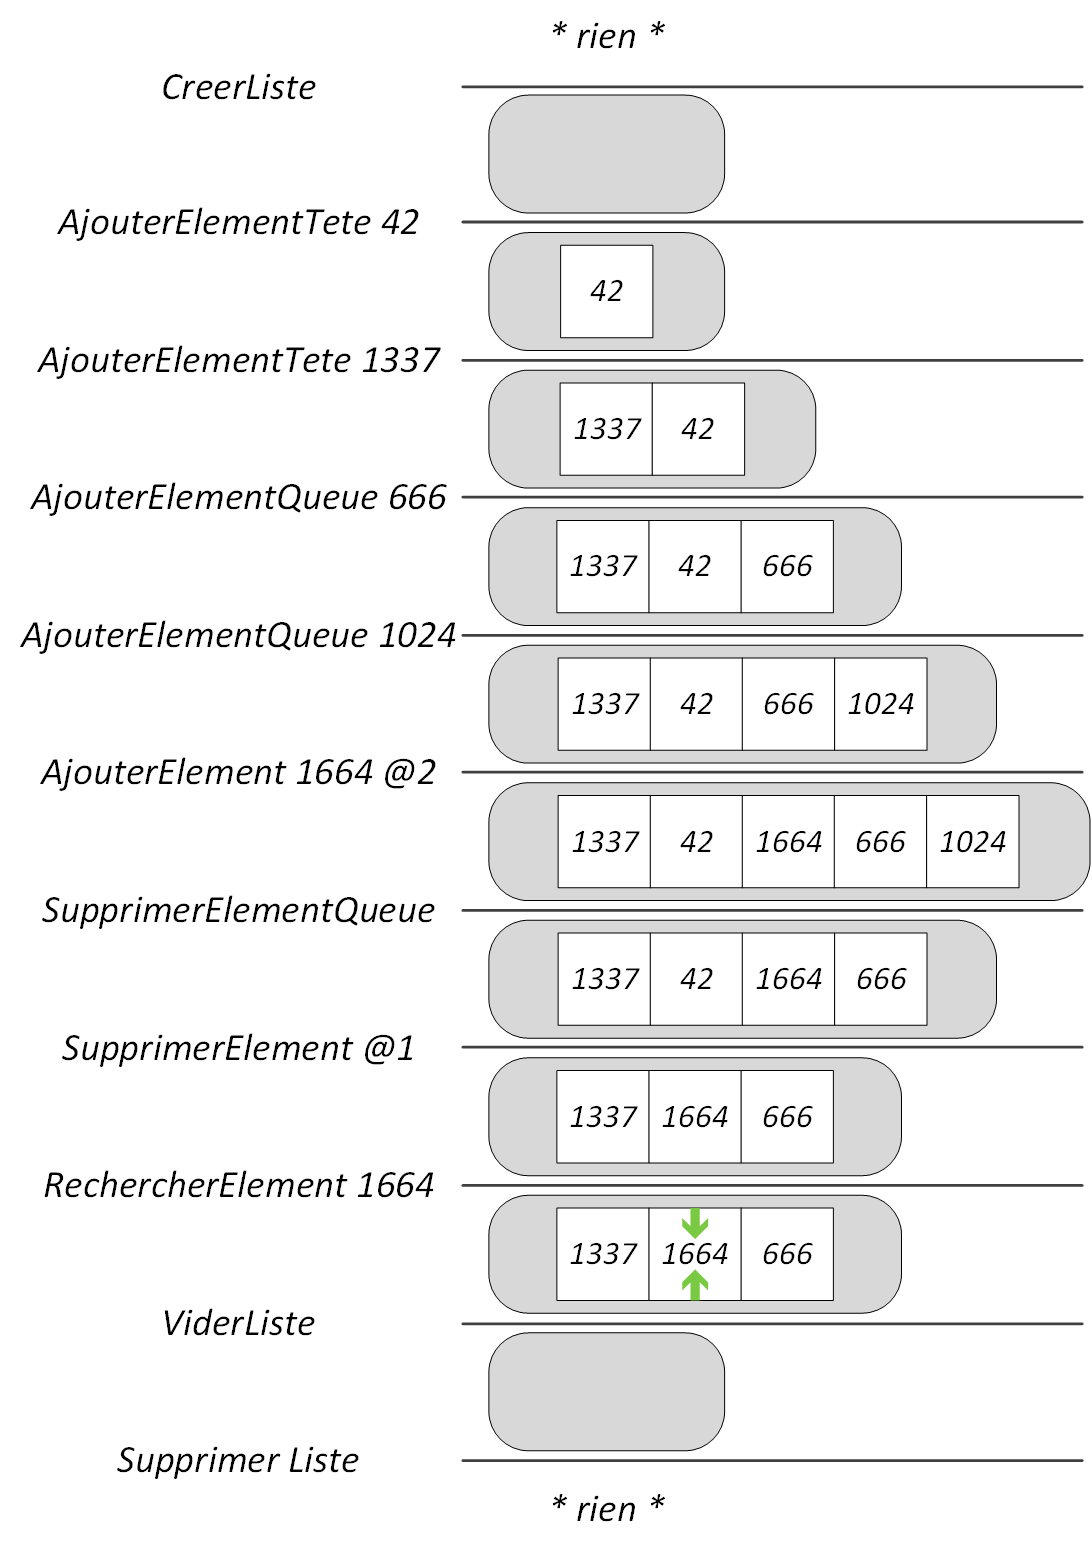
\includegraphics[scale=0.7]{img/listes/Listes_exemple1bis.png}
}
%\caption{Bubble Sort part 1}
%\label{figure:1-S3-DesignScience-ThreeLoops}
\end{figure}
%\end{figure*} % Figure flottante
% To use it : fig~\ref{label}

\end{center}

\bigskip

%%%%%%%%%%%%%%%%%%%

\subsection{Listes avec tableaux}

\bigskip

Parmi les implémentations possibles, on peut s'appuyer sur les tableaux.
Pour cela, on va définir au tout début un nombre maximal de cases dans lesquelles on pourra insérer des valeurs, et un nombre indiquant combien de valeurs sont actuellement stockées.

\begin{table}[h!]
  \centering
  \begin{minipage}{0.4\textwidth}
    \centering
% %*   *)
\begin{lstlisting}[style=algorithmique]
struct liste_t
  Elt[]   tab
  entier  max_len
  entier  nb_elt
fin struct \end{lstlisting}
    % \caption{Algorithme de la somme des N premiers entiers}
    % \label{algo-somme-n-premiers-entiers}
  \end{minipage}
  \hfillx
  \begin{minipage}{0.55\textwidth}
    \centering
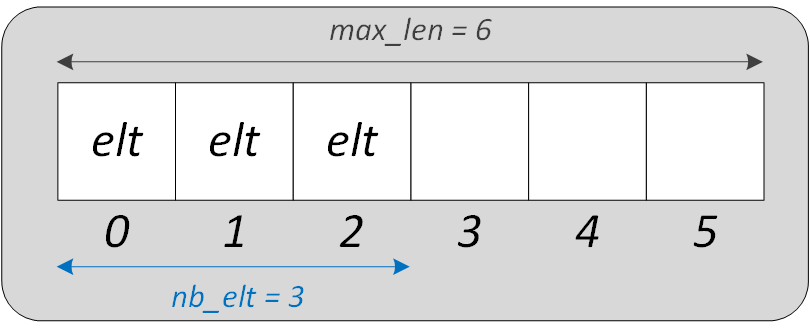
\includegraphics[scale=0.75]{img/listes/Listes_Tableau_1_Structure_Detaillee.png}
  \end{minipage}
%  \caption{Algorithme de la somme des N premiers entiers}
%  \label{somme-n-premiers-entiers}
\end{table}

Dans cette version, on peut effectivement ajouter des éléments n'importe où avec les algorithmes classiques vus précédemment (on décale tous les éléments dans un sens ou dans l'autre pour conserver le premier élément dans la case $ 0 $ du tableau).
Cette implémentation impose néanmoins une fonction supplémentaire à implémenter :

\begin{itemize}
\item \TTBF{TailleMaxListe(Liste) : entier}\\
      La fonction renvoie le nombre maximal d'éléments que peut stocker le tableau
\end{itemize}


Afin de se passer du nombre maximal d'éléments insérable dans le tableau, on peut imaginer un conteneur qui agrandit le tableau à chaque fois que l'espace vient à manquer, et qui libère l'espace en trop lorsque trop d'éléments ont été supprimés.
On peut fixer des limites selon les cas pratiques rencontrés, ou proposer diverses options à l'utilisateur (par exemple lors de la création de la liste, l'utilisateur peut indiquer le nombre initial de cases voulues, de combien les ajouts se feront, et au bout de quel pourcentage d'occupation on libèrera les cases en trop).


\bigskip

%%%%%%%%%%%%%%%%%%%

\subsection{Listes chaînées avec pointeurs}

\bigskip

En utilisant les pointeurs, on peut implémenter de façon plus générale encore les listes : on alloue de la mémoire pour chaque élément inséré, et on libère cette mémoire lors de la suppression de l'élément associé.
Le nombre maximum d'éléments que l'on pourra stocker dépendra exclusivement de la quantité de mémoire disponible et non plus de la taille de la structure algorithmique allouée.
Une autre différence majeure se situera dans la vitesse d'accès aux éléments : pour atteindre l'élément en position N, il est nécessaire de faire N déréférencements avant d'atteindre l'élément visé (et non plus renvoyer la case directement).

\medskip

En s'appuyant sur les pointeurs, chaque élément est en réalité une structure complète renvoyant éventuellement vers l'élément suivant OU signalant qu'il s'agit du dernier élément.
La création de la liste chaînée génèrera donc une structure vide qu'il faudra remplir par des ajouts successifs.
Cependant, nous allons implémenter une version extrêmement épurée de cette structure afin de mieux comprendre les pointeurs.
Dans ce cas précis, il n'y aura pas de fonction de création/suppression de la structure générale, mais uniquement des fonctions d'ajout et suppression d'éléments.
Ces fonctions d'ajout/suppression renverront à chaque fois le nouveau pointeur de tête de liste qu'il faut absolument conserver (si on perd ce pointeur, on perd l'adresse du premier élément, donc on ne peut plus le retrouver en mémoire et celui-ci sera définitivement alloué/impossible à réutiliser par le système et d'autres programmes).

\begin{table}[h!]
  \centering
  \begin{minipage}{0.4\textwidth}
    \centering
% %*   *)
\begin{lstlisting}[style=algorithmique]
struct liste_p
  Elt      elt
  liste_p  *next
fin struct \end{lstlisting}
    % \caption{Algorithme de la somme des N premiers entiers}
    % \label{algo-somme-n-premiers-entiers}
  \end{minipage}
  \hfillx
  \begin{minipage}{0.55\textwidth}
    \centering
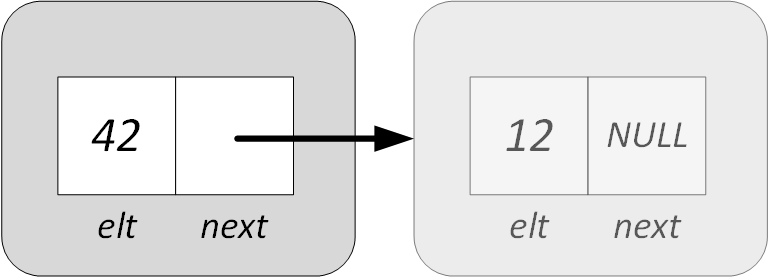
\includegraphics[scale=0.75]{img/listes/Listes_Pointeurs_1_Structure_Detaillee.png}
  \end{minipage}
%  \caption{Algorithme de la somme des N premiers entiers}
%  \label{somme-n-premiers-entiers}
\end{table}

Ainsi, on peut trouver 3 cas possibles :
\begin{itemize}
\item \textit{la liste est vide} : le pointeur de liste est à \TTBF{NULL}
\item \textit{la liste contient un seul élément (le premier qui est aussi le dernier)} : le pointeur de liste pointe vers une structure en mémoire, dont le champs \TTBF{next} est à la valeur \TTBF{NULL}
\item \textit{la liste contenant N éléments} : le pointeur de liste pointe vers une structure qui est le premier élément, et son champs \TTBF{next} contient une valeur qui n'est pas \TTBF{NULL}
\end{itemize}

\medskip

%\begin{figure*} % Figure flottante
\begin{figure}[ht!]
\centering
\centerline{   % width=1.18\textwidth  grand grand max
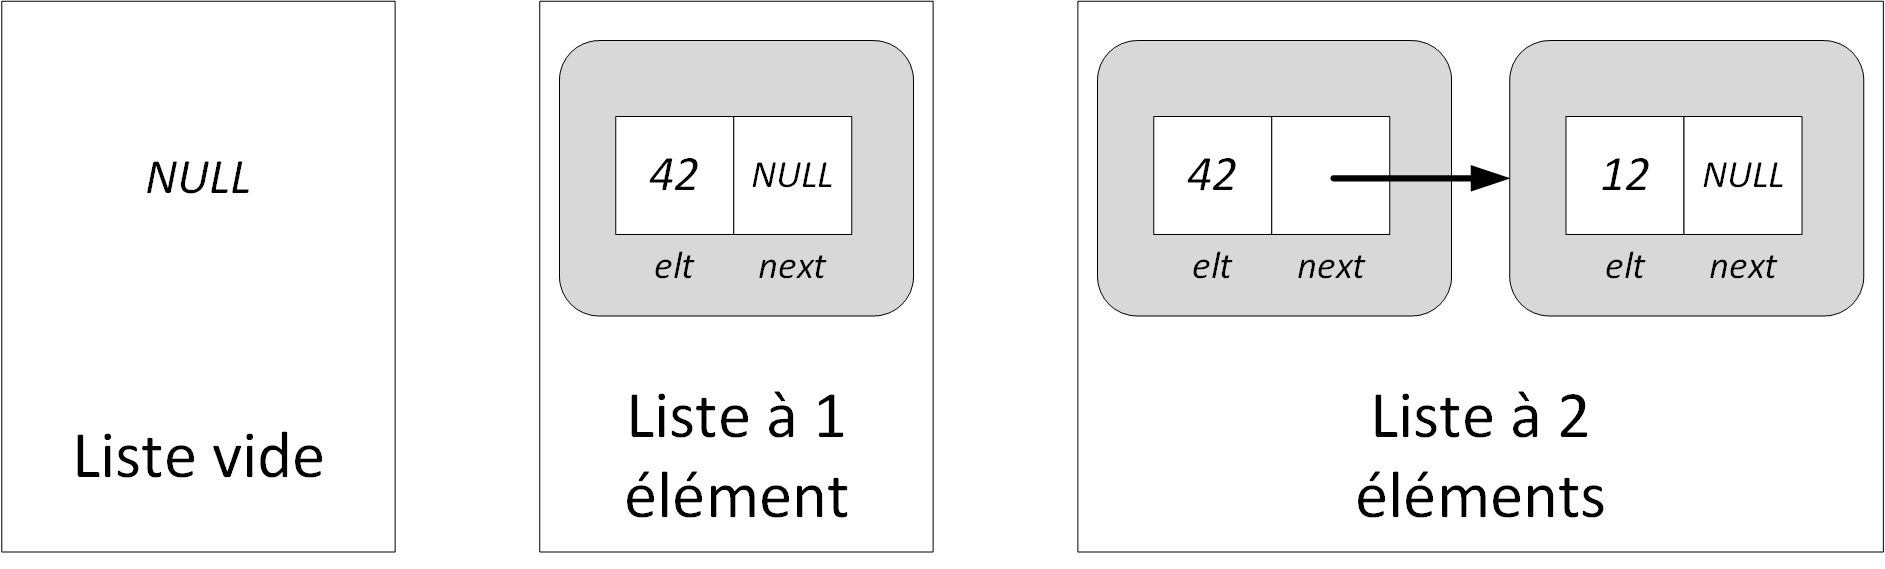
\includegraphics[width=0.85\textwidth]{img/listes/Listes_Pointeurs_2_exemple1_espace.png}
}
%\caption{Bubble Sort part 1}
%\label{figure:1-S3-DesignScience-ThreeLoops}
\end{figure}
%\end{figure*} % Figure flottante
% To use it : fig~\ref{label}

\medskip

Parmi les fonctions à implémenter pour cette structure précise, on devra donc écrire :

\begin{itemize}
\item \TTBF{AjouterElement(Liste, Elt, Pos) : Liste}\\
      La fonction essaye d'ajouter un élément \textit{Elt} à l'index \textit{Pos} de la liste \textit{Liste}. Si la liste est vide (la valeur du pointeur est \TTBF{NULL}), alors on alloue juste un élément et on renvoie son adresse. Si un élément est déjà présent à cette position, il est poussé un cran vers la queue de la liste, et on ajoute le nouvel élément à son ancienne place (on met à jour le pointeur de l'élément précédent, et le nouvel élément pointe vers l'ancien). On renverra le pointeur de la tête de liste (au cas où l'on insère un élément en tête).
\item \TTBF{SupprimerElement(Liste, Pos) : booléen}\\
      La fonction essaye de supprimer l'élément présent à l'index \textit{Pos} de la liste \textit{Liste}. Elle renvoie le pointeur de la nouvelle tête de liste en cas de succès (éventuellement \textit{NULL} si la liste devient vide). On renverra la tête de liste actuelle si la position supprimée n'existe pas.
\item \textit{[AjouterElementTete, AjouterElementQueue, AjouterElementMilieu, SupprimerElementTete, SupprimerElementQueue, SupprimerElementMilieu sont les 6 algorithmes avec des cas spécifiques utilisés pour l'ajout et la suppression]}
\item \TTBF{ViderListe(Liste) : entier}\\
      La fonction supprime tous les éléments contenus dans la liste. Puis elle renvoie le nombre d'éléments supprimés
\item \TTBF{TailleListe(Liste) : entier}\\
      La fonction renvoie la taille de la liste, c'est-à-dire le nombre d'éléments présents dedans
\item \TTBF{RechercherElement(Liste, Elt) : entier}\\
      La fonction cherche un élément \textit{Elt} dans la liste \textit{Liste}, puis renvoie l'index de sa position (on considère que le premier élément est $ 0 $), ou $ -1 $ si l'élément n'est pas trouvé
\item \TTBF{RecupererElement(Liste, Pos) : [type Elt]}\\
      La fonction récupère l'élément présent à l'index \textit{Pos} de la liste \textit{Liste} et le renvoie (vous renverrez l'entier qui est contenu dans le champ \textit{elt} de la structure). S'il n'est pas trouvé, vous renverrez une valeur d'erreur (c'est-à-dire $ -1 $ dans notre cas)
\end{itemize}

\bigskip

Pour bien comprendre l'ajout d'un élément, voici les différents cas illustrés :

\vfillFirst

%\begin{figure*} % Figure flottante
\begin{figure}[ht!]
\centering
\centerline{   % width=0.85\textwidth OK  width=1.18\textwidth  grand grand max
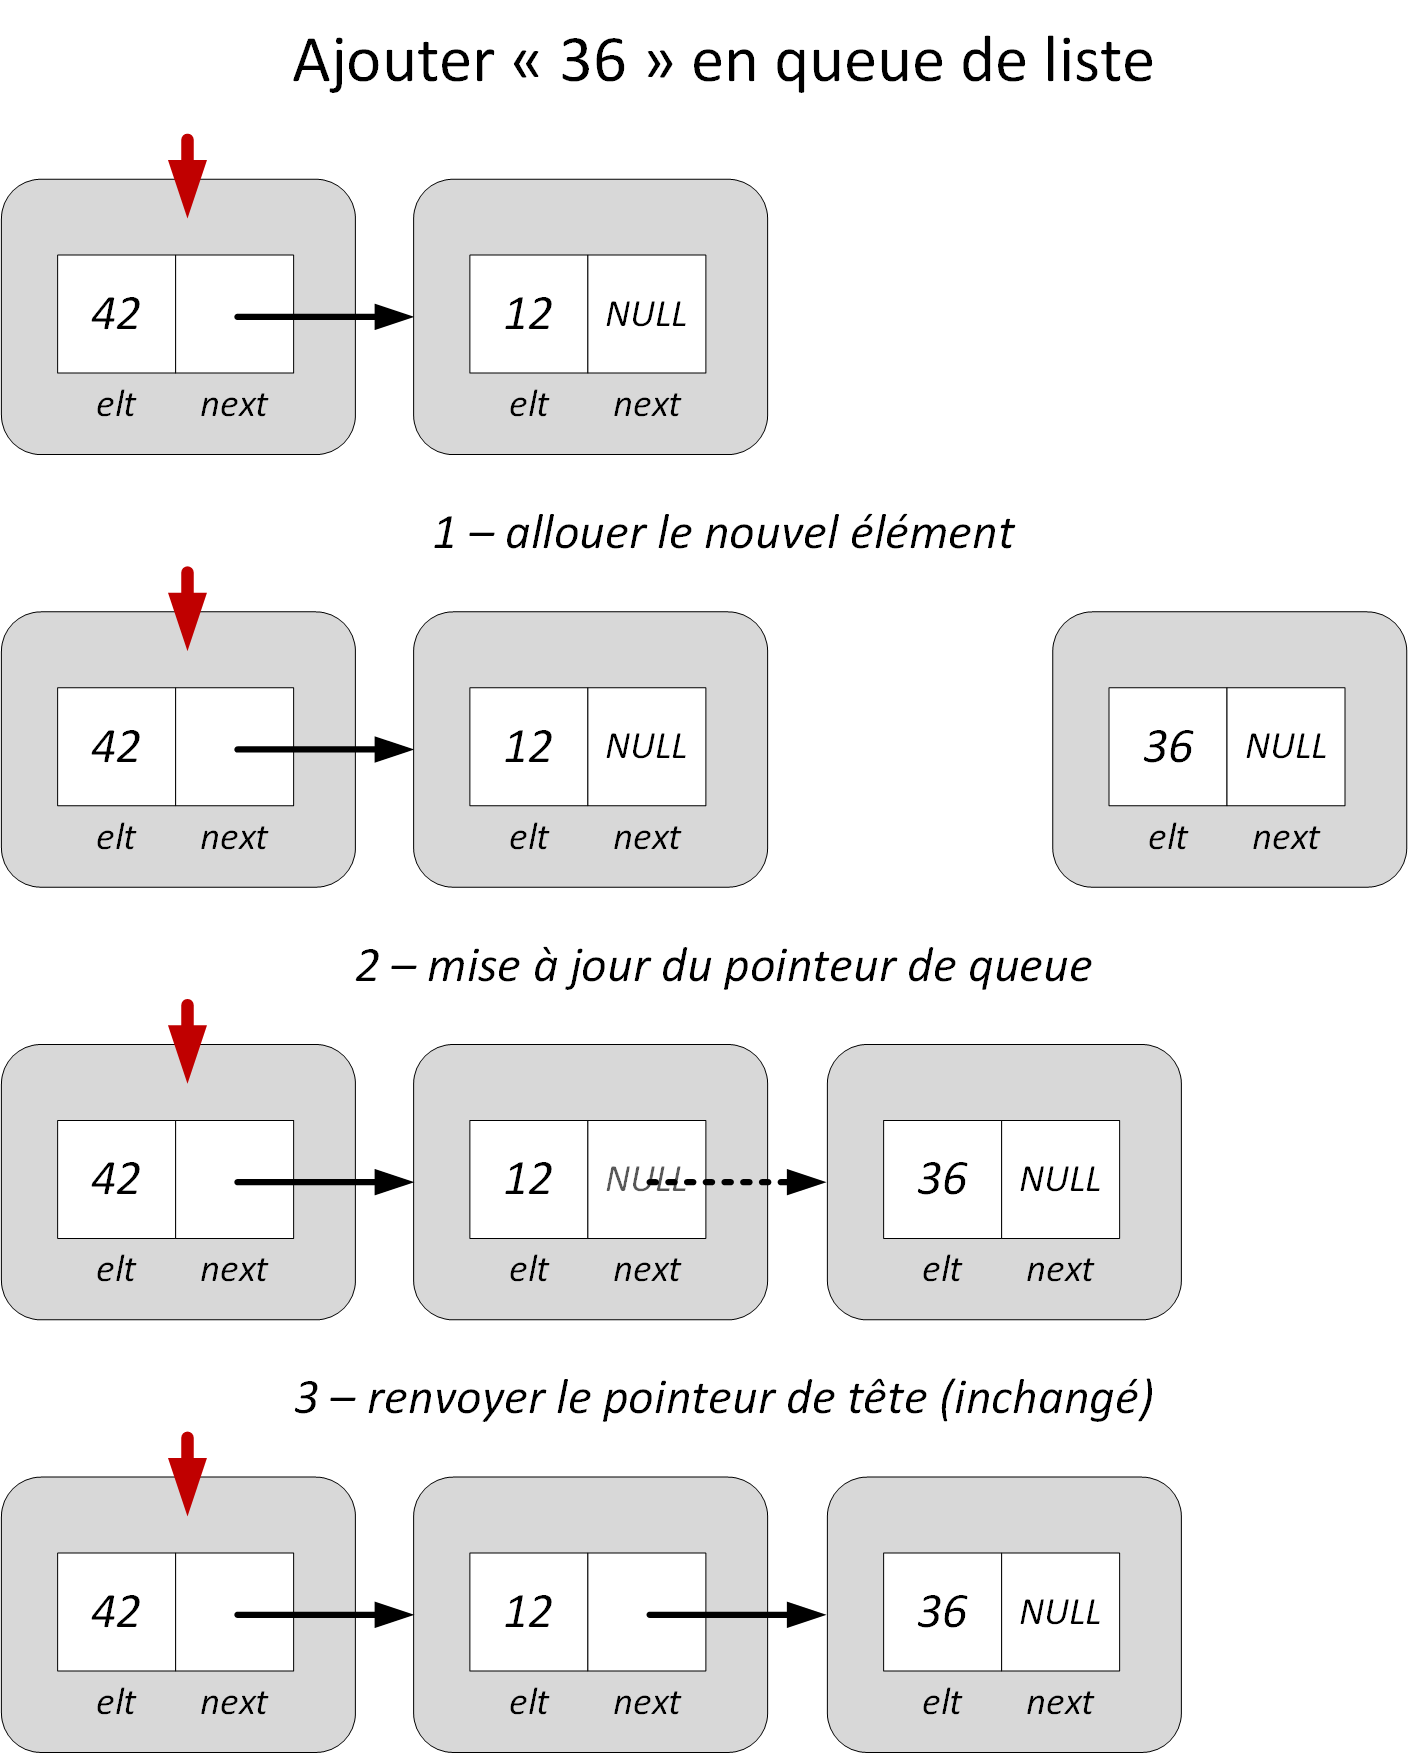
\includegraphics[scale=0.85]{img/listes/Listes_Pointeurs_3_1_ajout_queue.png}
}
%\caption{Bubble Sort part 1}
%\label{figure:1-S3-DesignScience-ThreeLoops}
\end{figure}
%\end{figure*} % Figure flottante
% To use it : fig~\ref{label}

\vfillLast

\pagebreak

\vfillFirst

%\begin{figure*} % Figure flottante
\begin{figure}[ht!]
\centering
\centerline{   % width=0.85\textwidth OK  width=1.18\textwidth  grand grand max
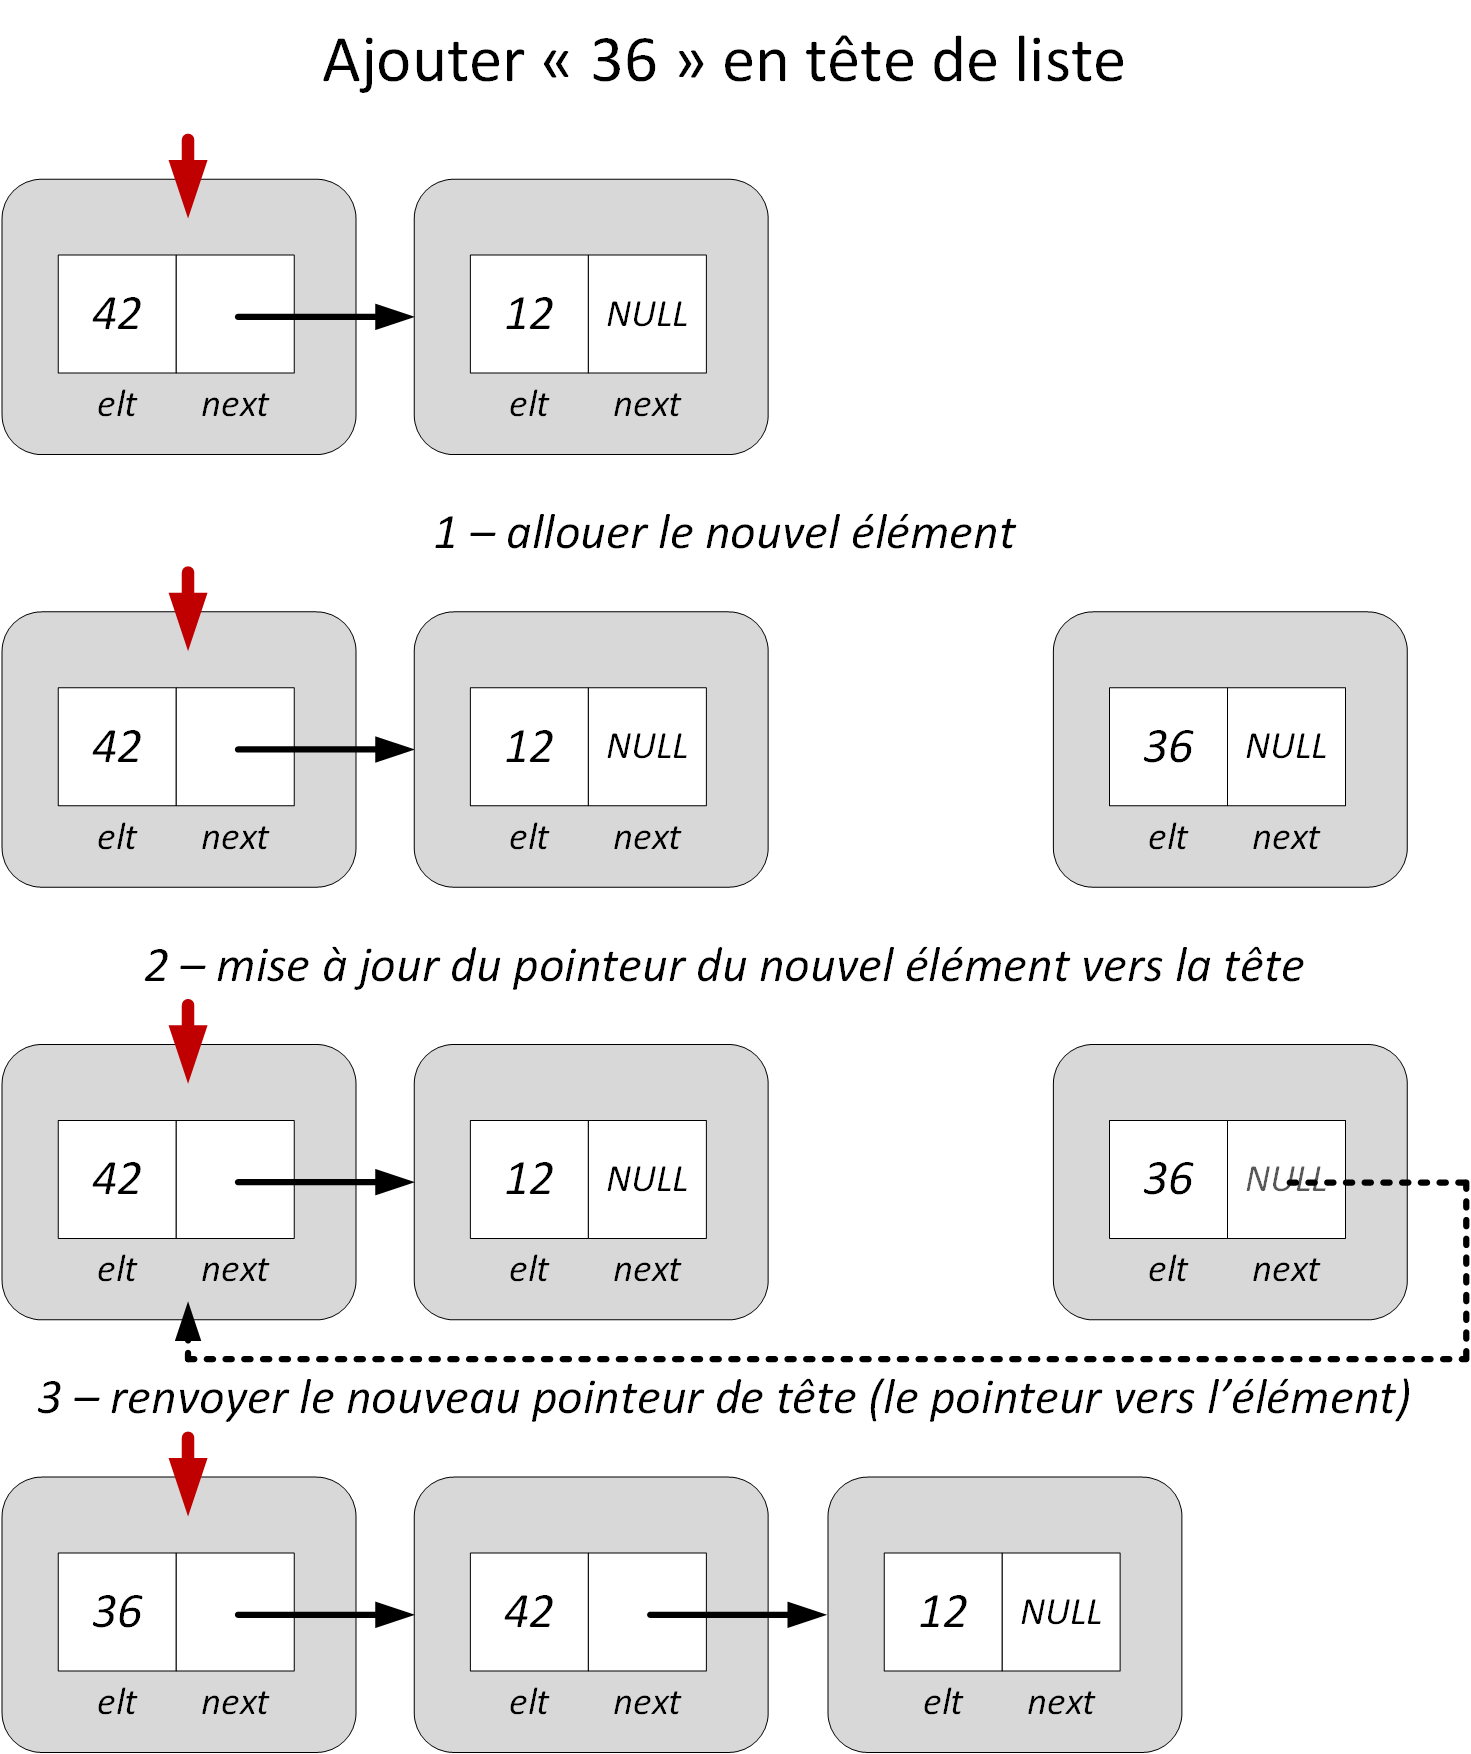
\includegraphics[scale=0.85]{img/listes/Listes_Pointeurs_3_3_ajout_tete.png}
}
%\caption{Bubble Sort part 1}
%\label{figure:1-S3-DesignScience-ThreeLoops}
\end{figure}
%\end{figure*} % Figure flottante
% To use it : fig~\ref{label}

\vfillLast

\pagebreak

\vfillFirst

%\begin{figure*} % Figure flottante
\begin{figure}[ht!]
\centering
\centerline{   % width=0.85\textwidth OK  width=1.18\textwidth  grand grand max
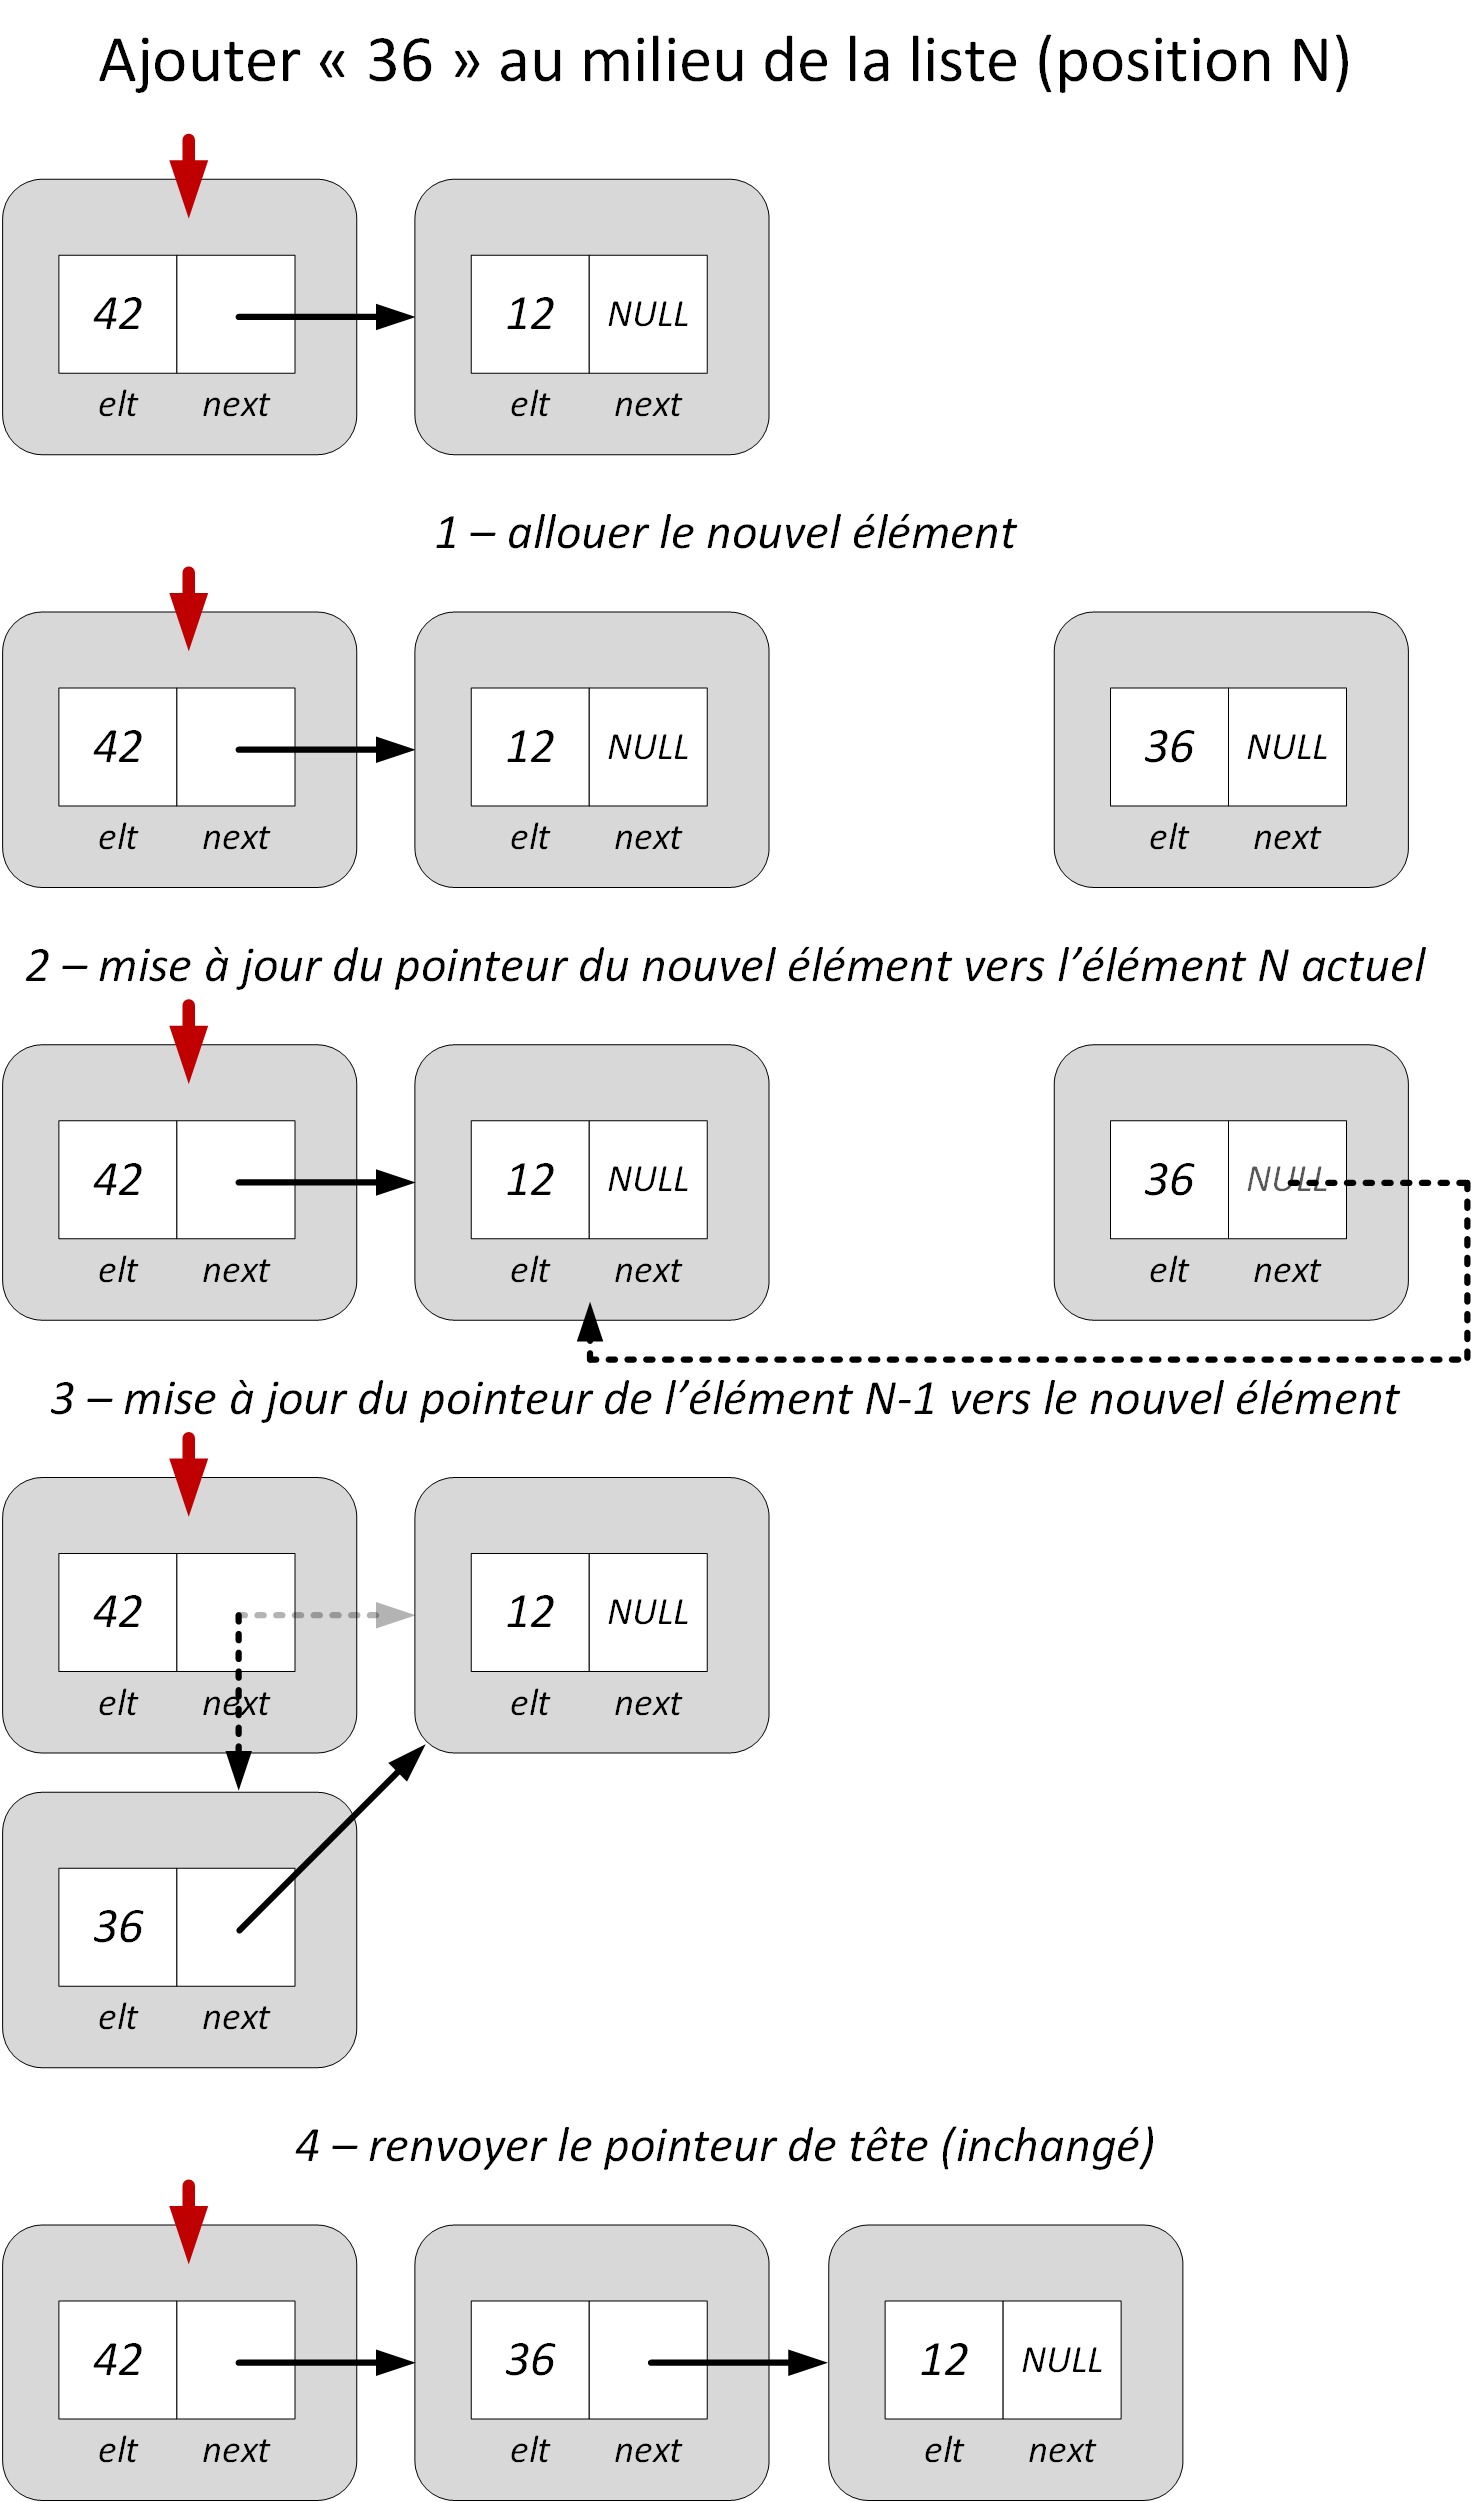
\includegraphics[scale=0.73]{img/listes/Listes_Pointeurs_3_2_ajout_milieu.png}
}
%\caption{Bubble Sort part 1}
%\label{figure:1-S3-DesignScience-ThreeLoops}
\end{figure}
%\end{figure*} % Figure flottante
% To use it : fig~\ref{label}

\vfillLast

\pagebreak

De même, la suppression implique des mises à jour sur plusieurs pointeurs :

\vfillFirst

%\begin{figure*} % Figure flottante
\begin{figure}[ht!]
\centering
\centerline{   % width=0.85\textwidth OK  width=1.18\textwidth  grand grand max
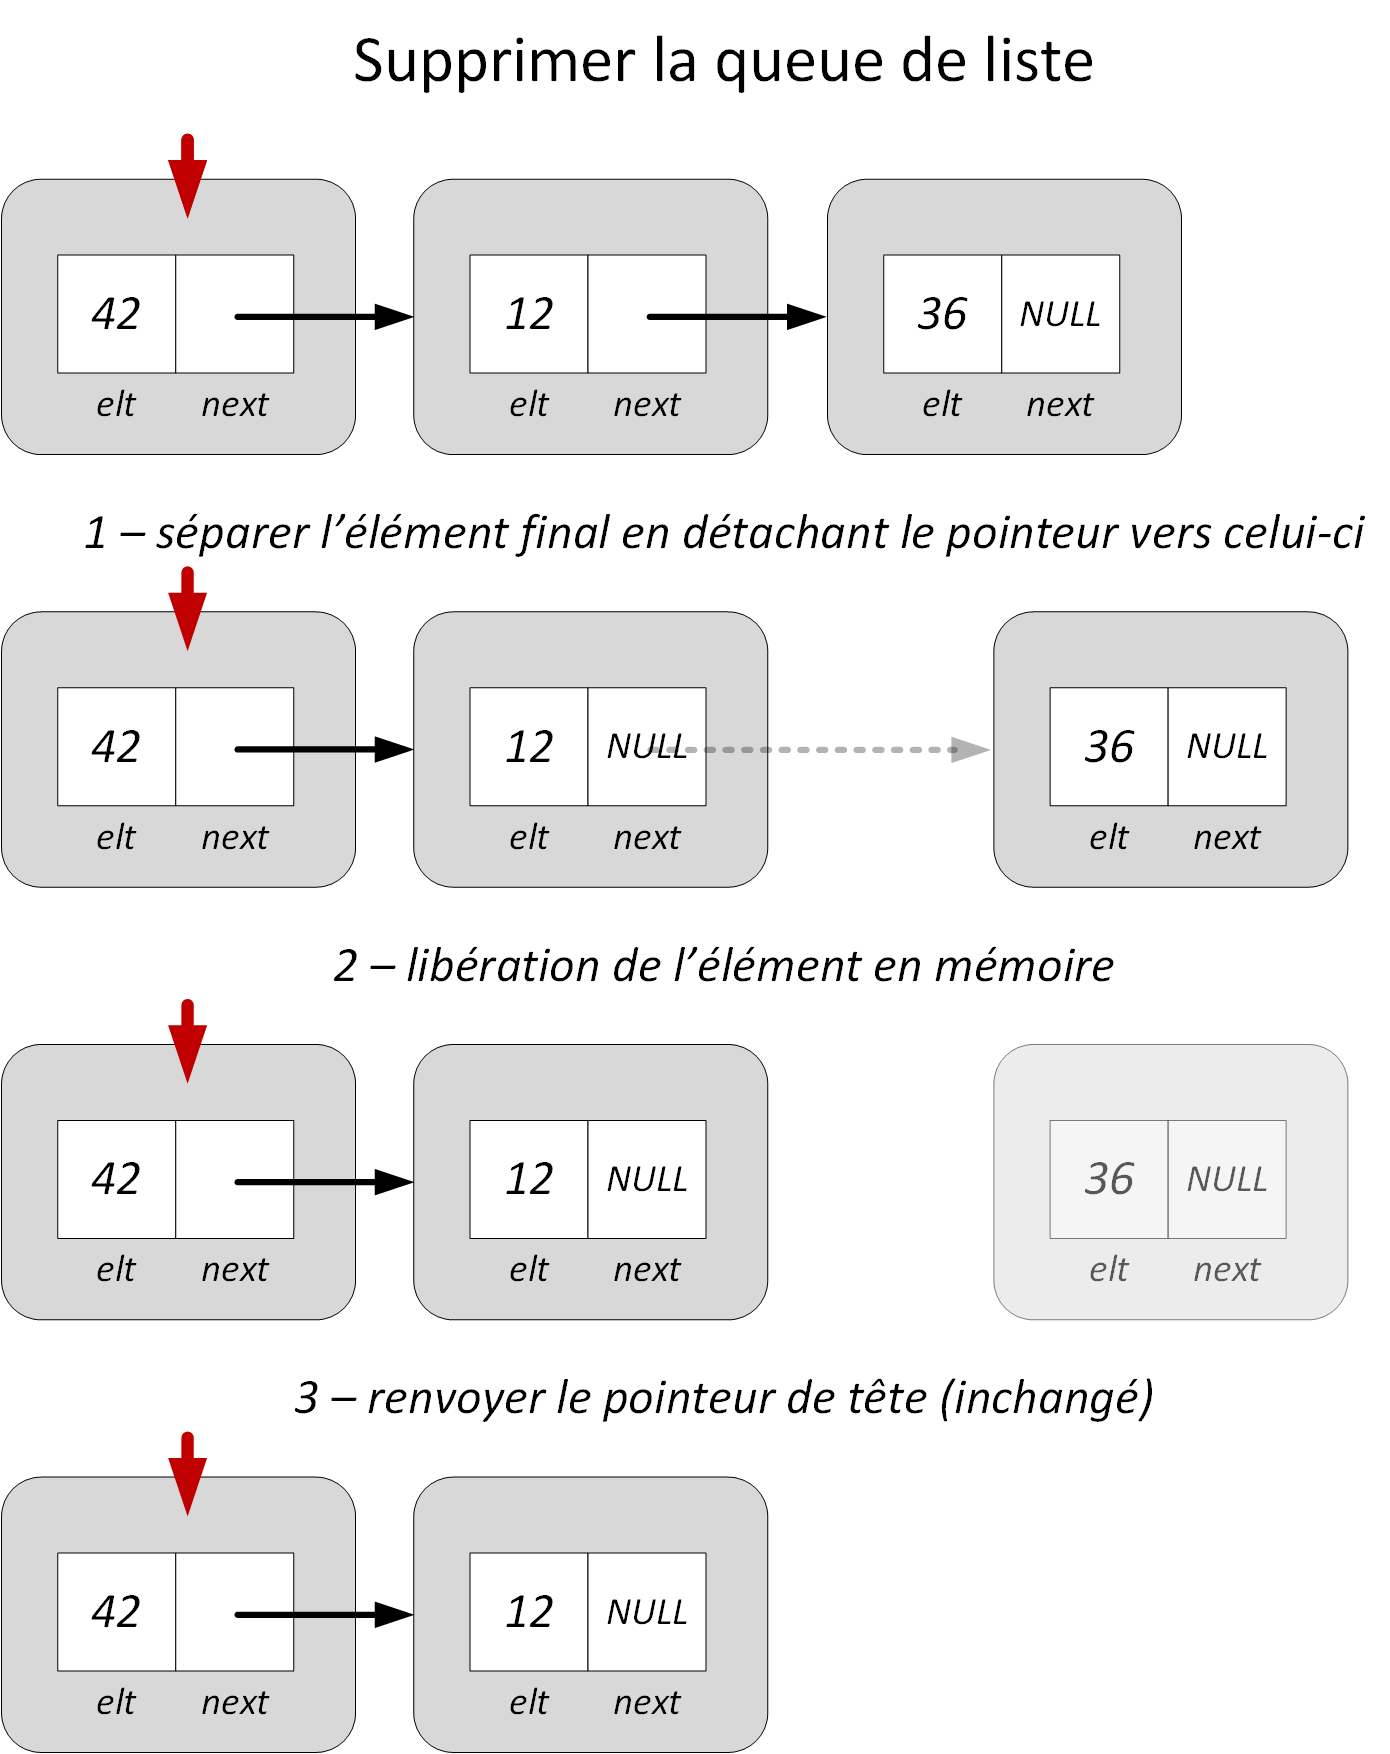
\includegraphics[scale=0.85]{img/listes/Listes_Pointeurs_4_1_suppression_queue.png}
}
%\caption{Bubble Sort part 1}
%\label{figure:1-S3-DesignScience-ThreeLoops}
\end{figure}
%\end{figure*} % Figure flottante
% To use it : fig~\ref{label}

\vfillLast

\pagebreak

\vfillFirst

%\begin{figure*} % Figure flottante
\begin{figure}[ht!]
\centering
\centerline{   % width=0.85\textwidth OK  width=1.18\textwidth  grand grand max
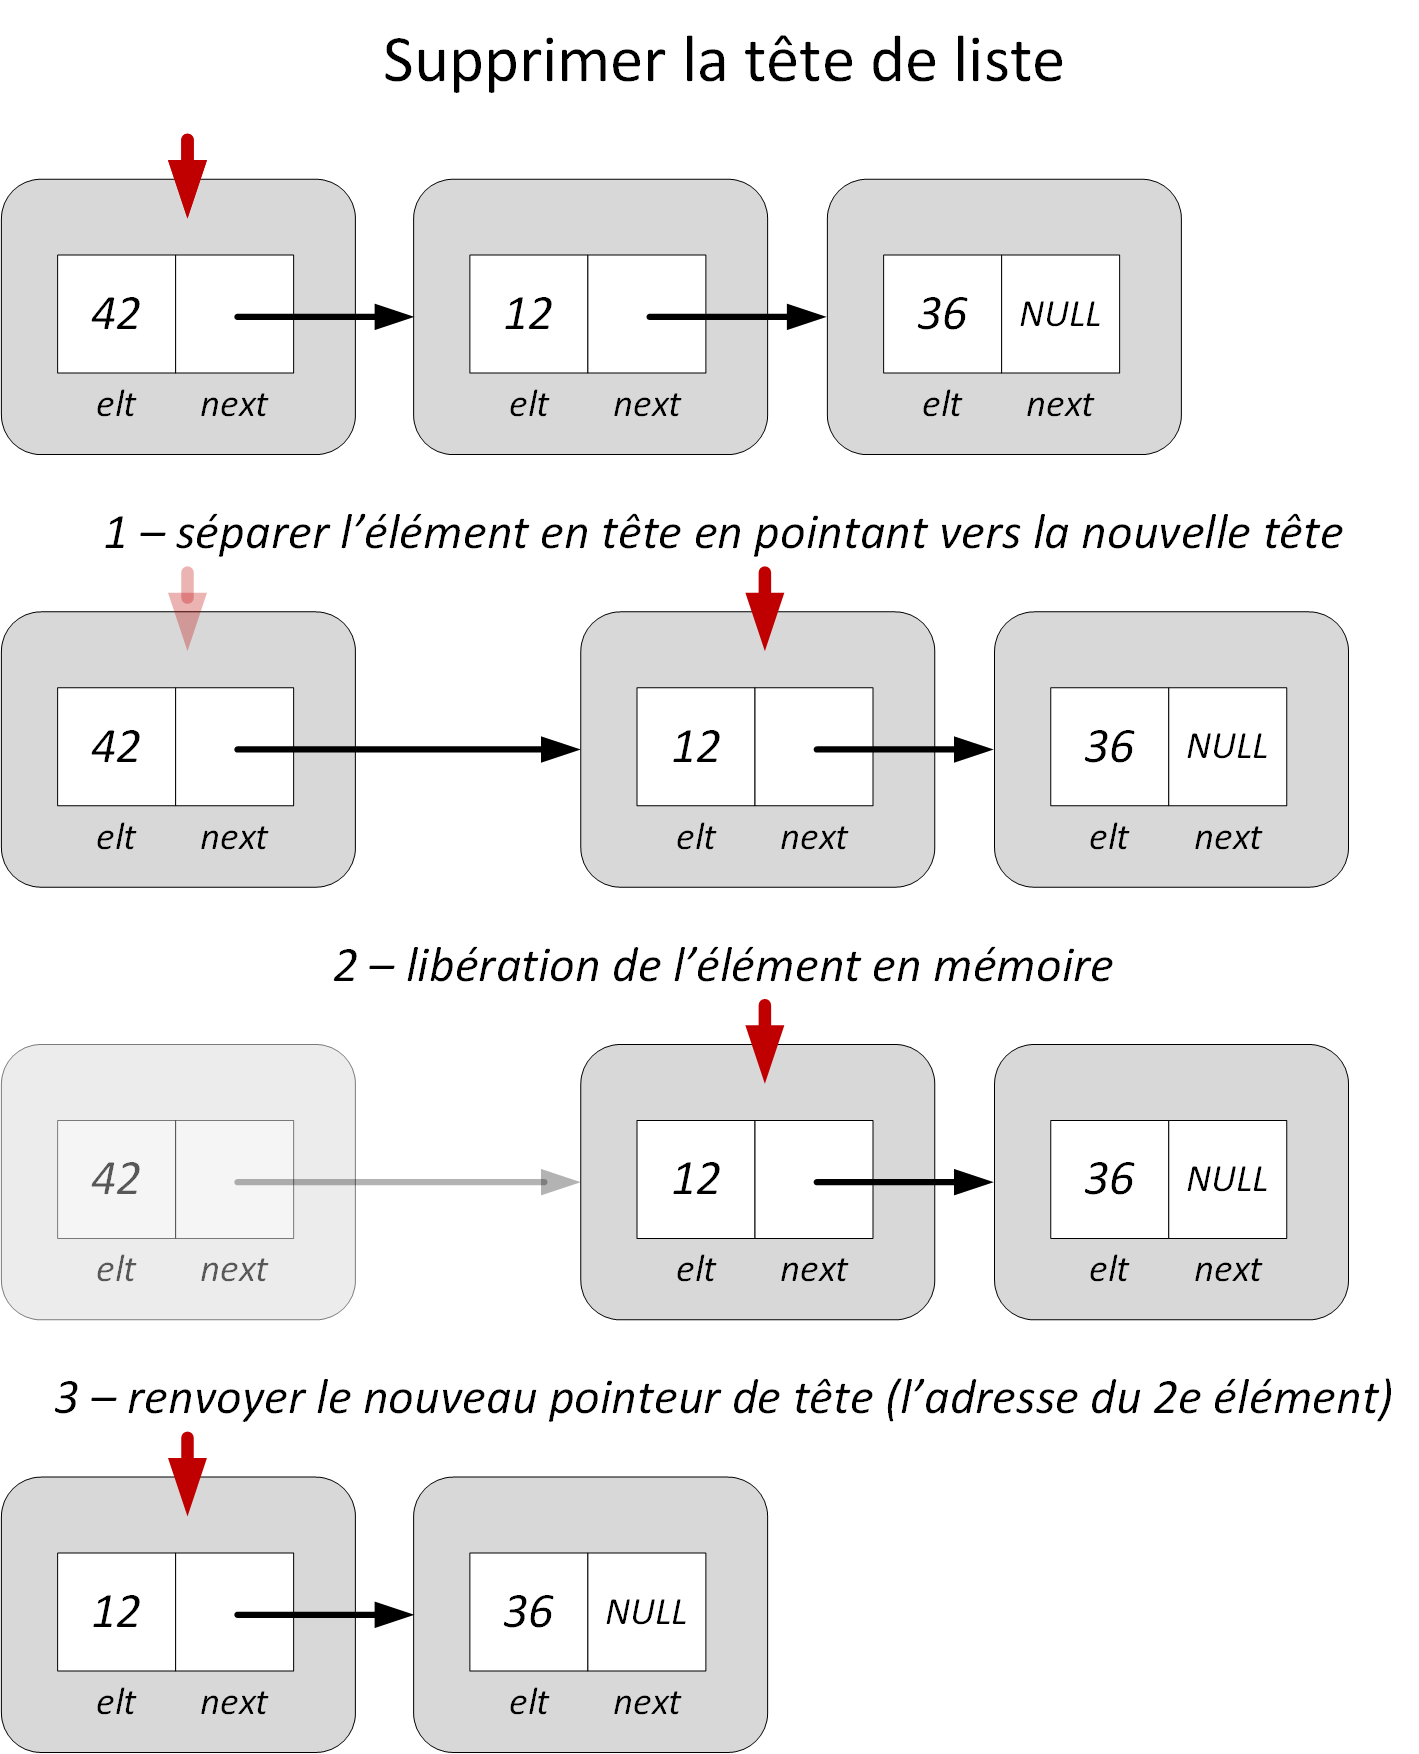
\includegraphics[scale=0.85]{img/listes/Listes_Pointeurs_4_2_suppression_tete.png}
}
%\caption{Bubble Sort part 1}
%\label{figure:1-S3-DesignScience-ThreeLoops}
\end{figure}
%\end{figure*} % Figure flottante
% To use it : fig~\ref{label}

\vfillLast

\pagebreak

\vfillFirst

%\begin{figure*} % Figure flottante
\begin{figure}[ht!]
\centering
\centerline{   % width=0.85\textwidth OK  width=1.18\textwidth  grand grand max
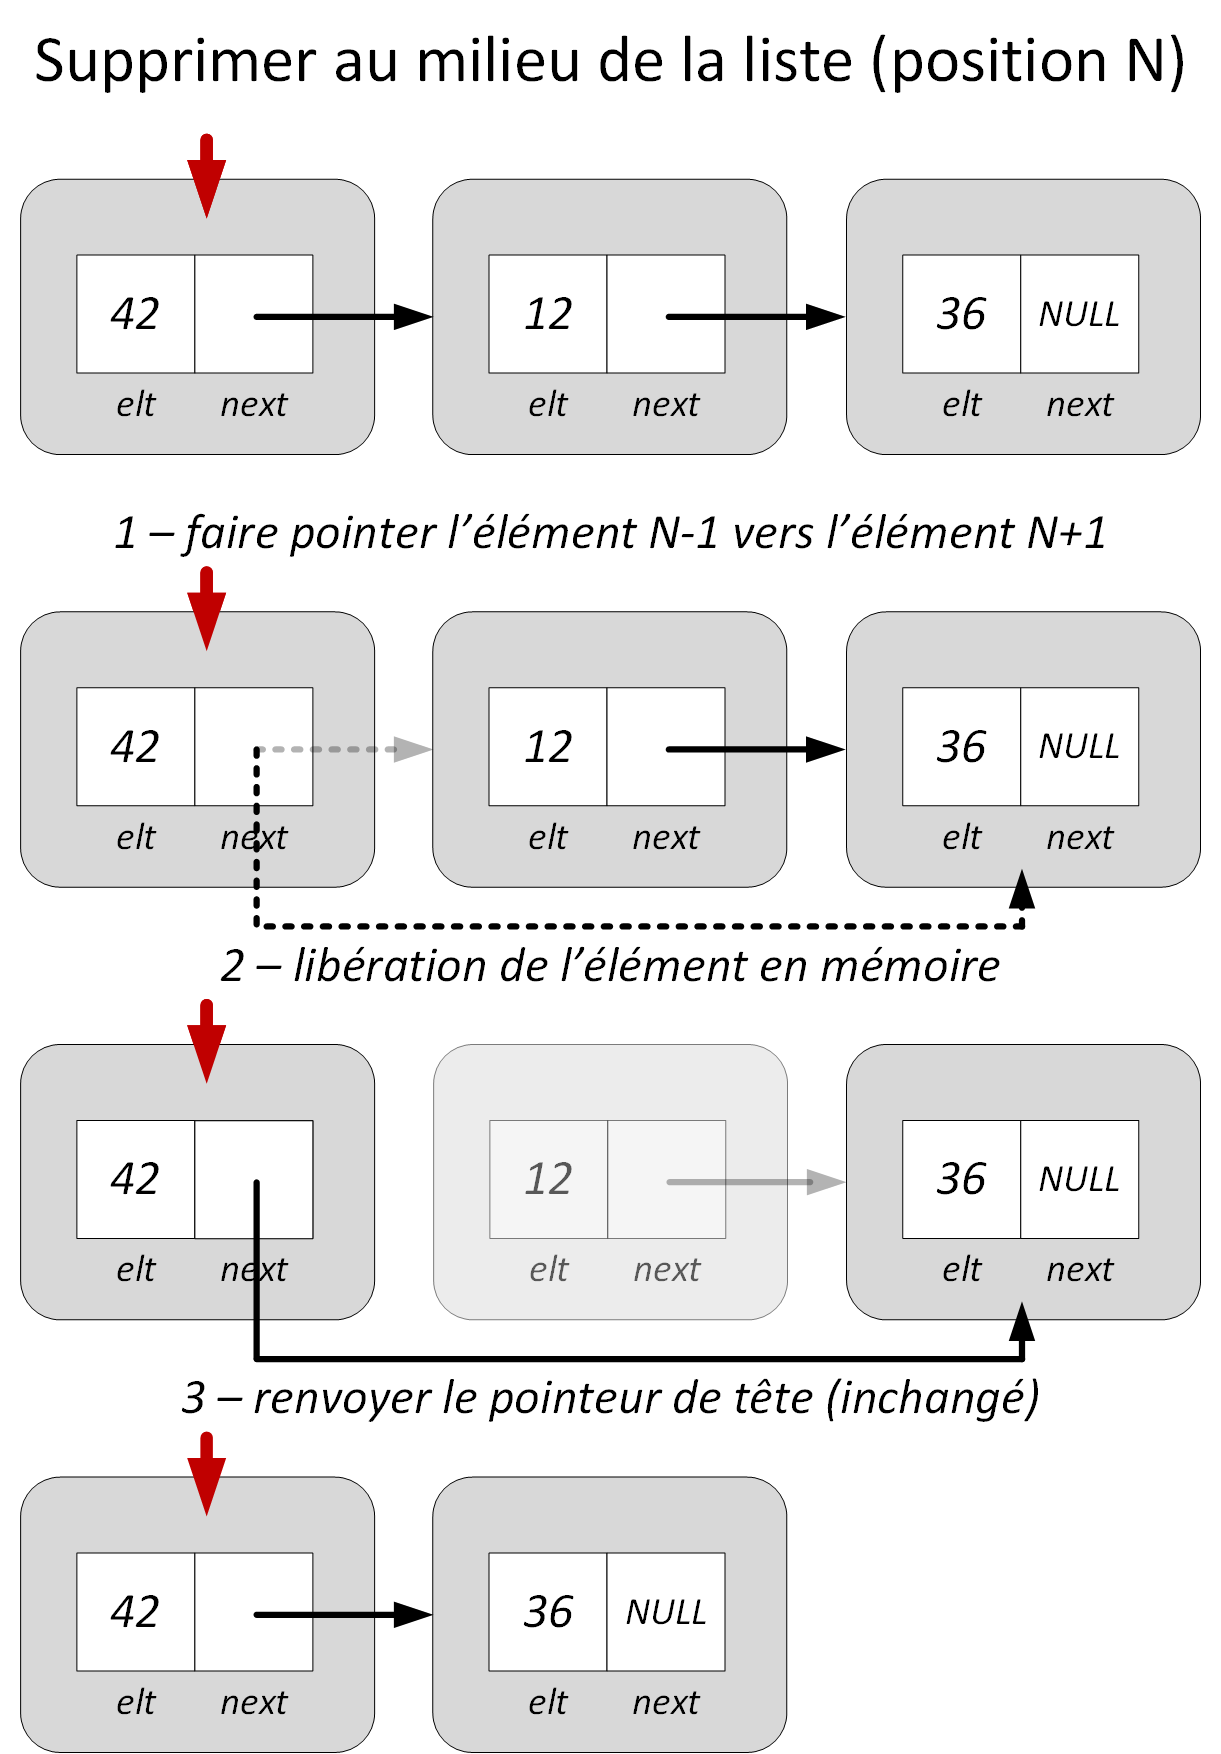
\includegraphics[scale=0.85]{img/listes/Listes_Pointeurs_4_3_suppression_milieu.png}
}
%\caption{Bubble Sort part 1}
%\label{figure:1-S3-DesignScience-ThreeLoops}
\end{figure}
%\end{figure*} % Figure flottante
% To use it : fig~\ref{label}

\vfillLast


\newpage

%%%%%%%%%%%%%%%%%%%%%%%%%%%%%%%%%%%%%%

\section{Piles}

\bigskip

Les \textbf{piles}, ou \textbf{stacks} en anglais, sont des structures visant à stocker les données dans l'ordre d'arrivée, mais ne permettant leur récupération uniquement dans l'ordre inverse.
Dans une pile, on ne peut accéder qu'à la dernière donnée stockée, celle se situant au \textit{sommet} de la pile.
Ces structures sont aussi appelées \textbf{LIFO} (\textit{Last In First Out}).\\

\begin{center}
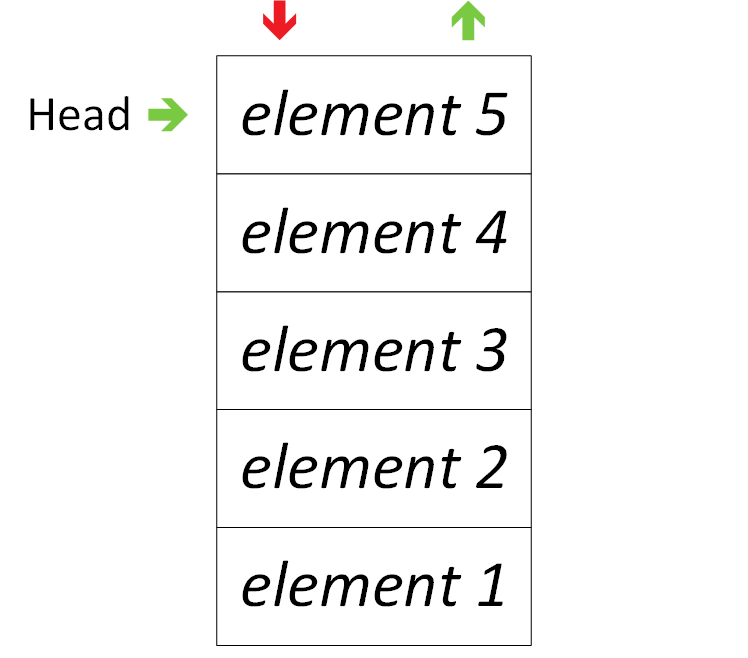
\includegraphics[scale=0.75]{img/piles/Piles_1_Structure_Generale_centered.png}
\end{center}

\smallskip

Deux opérations permettent d'utiliser une pile :
\begin{itemize}
\item \TTBF{PUSH} : permettant d'\textit{empiler} une donnée supplémentaire dans la pile
\item \TTBF{POP} : permettant de \textit{dépiler} une donnée depuis la pile
\end{itemize}
On ajoute donc une donnée en l'empilant avec un \TTBF{PUSH}, et il est possible de directement y accéder, car elle est au sommet de la pile.
À l'inverse, pour accéder à une donnée tout au fond de la pile, il est nécessaire de dépiler autant d'éléments que nécessaire avec un \TTBF{POP}.\\

Voici un exemple où l'on crée une pile, puis on empile successivement $ 42 $, $ 5 $, et $ 13 $, puis, on dépile une fois (pour récupérer $ 13 $), et enfin, on empile successivement $ 37 $, $ 10 $, $ 24 $.\\

\vfillFirst

\begin{center}
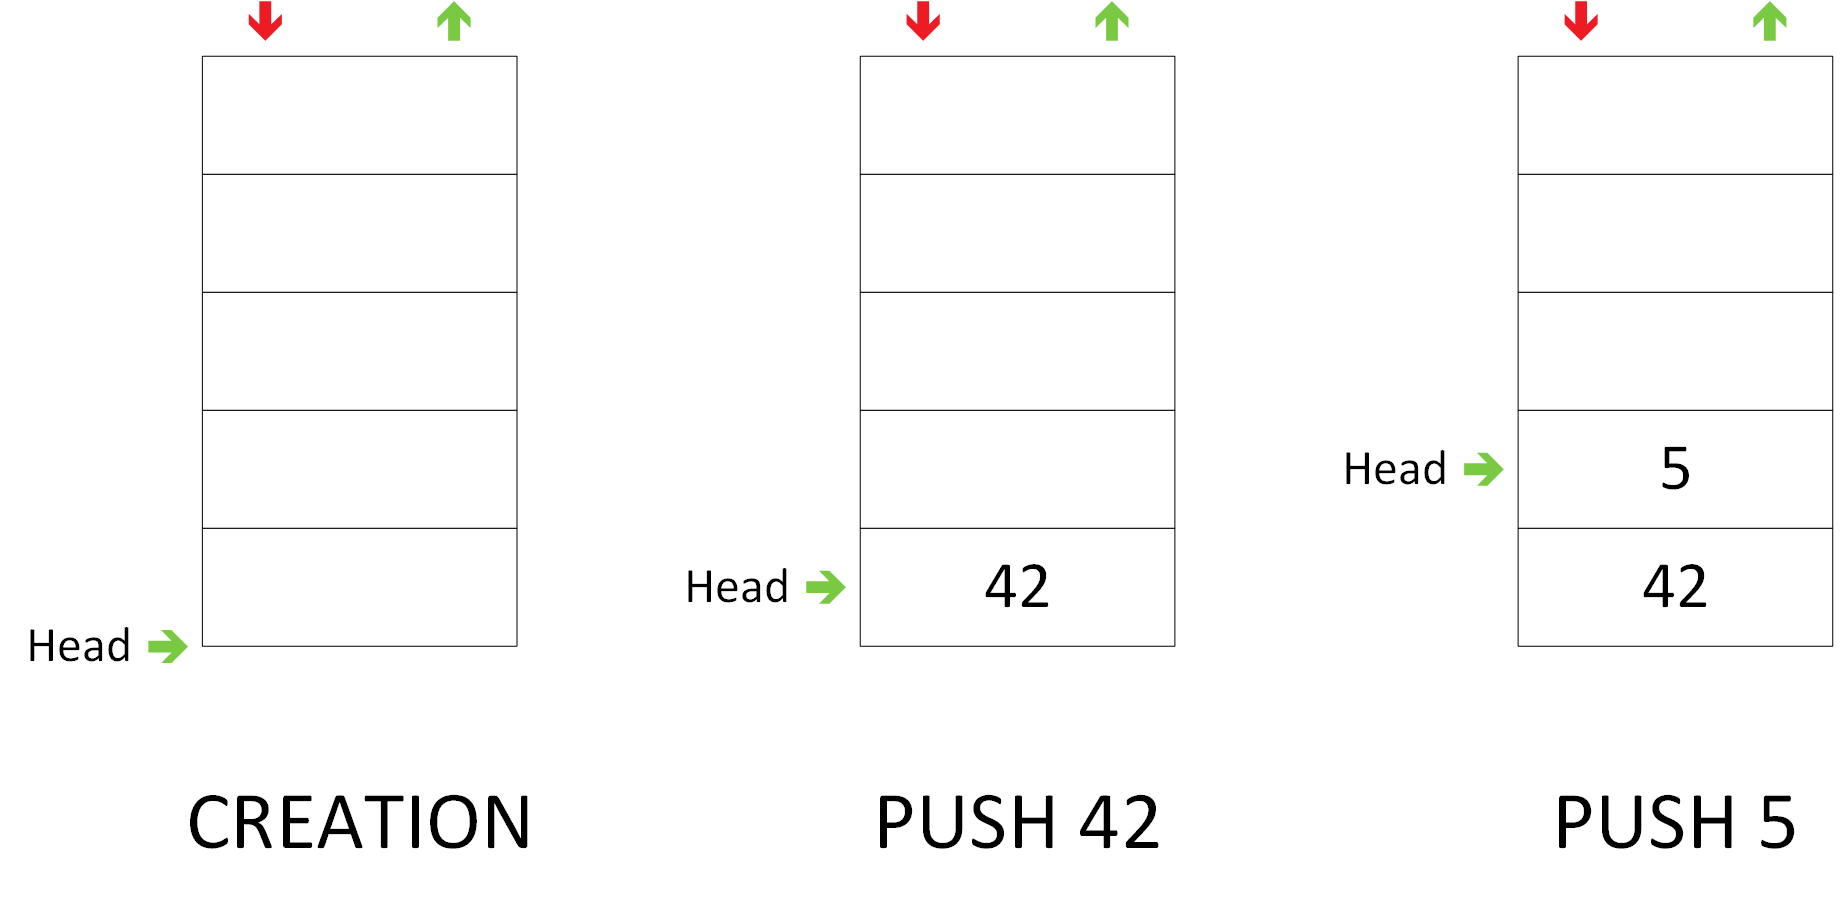
\includegraphics[scale=0.5]{img/piles/Piles_2_Structure_Generale_Usage_pack_1.png}
\end{center}

\vfillLast

\pagebreak

\begin{center}
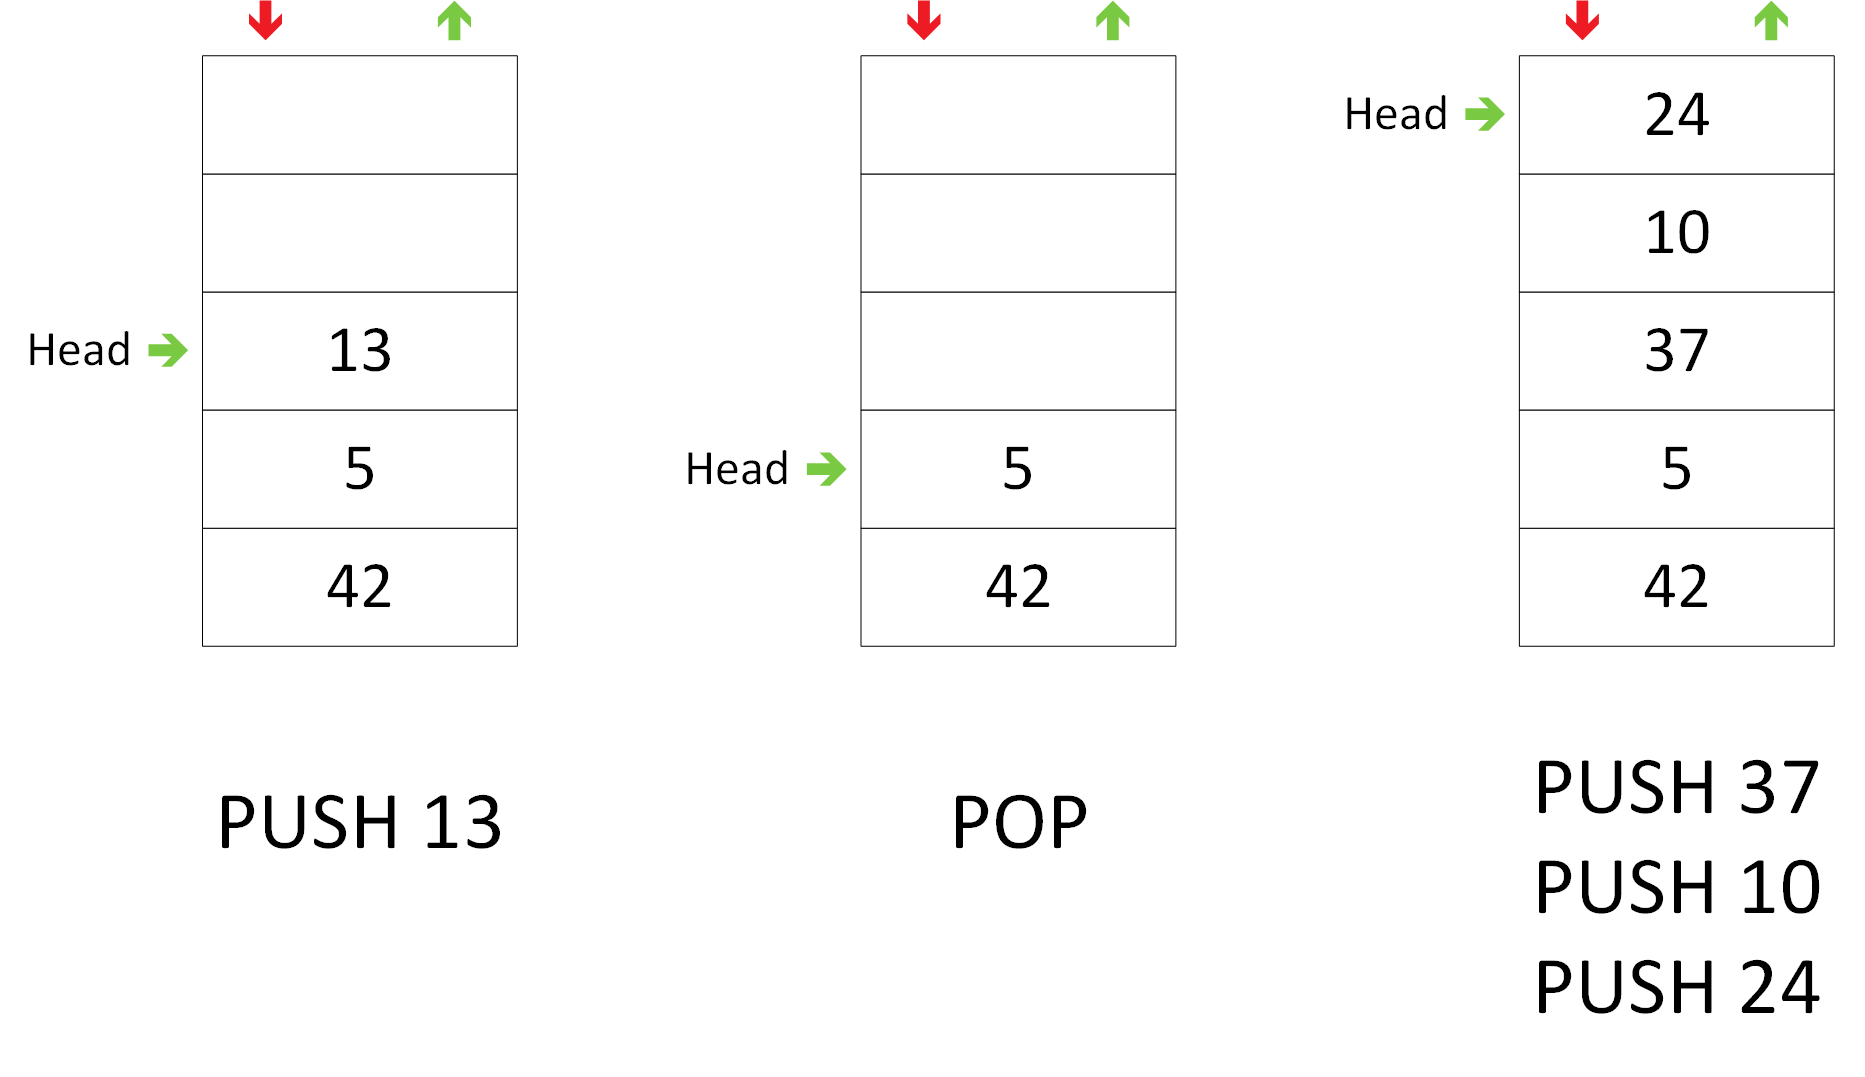
\includegraphics[scale=0.5]{img/piles/Piles_2_Structure_Generale_Usage_pack_2.png}
\end{center}

\smallskip

Les piles, et surtout la contrainte d'accès aux objets, sont couramment utilisées : un camion de livraison sera d'abord rempli avec les paquets à livrer en dernier/le camion sera rempli dans l'ordre inverse de livraison (on accède d'abord aux derniers éléments chargés).

En informatique, on utilisera les piles dans certains \textit{parsers} (analyse grammaticale) pour connaître en premier l'opérateur à exécuter (opérateur binaire ? unaire ?) et dépiler par la suite le nombre exact de paramètres.
La \textit{pile d'appels} est également une convention fondamentale partagée par les processeurs et les systèmes d'exploitation permettant de passer des paramètres (et d'autres informations de contexte) aux fonctions appelées par les programmes, ou en cas d'interruption pour sauvegarder l'adresse de l'instruction qui était en cours d'exécution.\\

Afin d'implémenter une pile, il est donc nécessaire d'avoir un espace de stockage ordonné (un tableau numéroté ou une liste chaînée), et un indicateur de l'élément en haut de la pile.
Nous allons maintenant voir comment implémenter une pile avec des listes chaînées et un tableau de taille fixe.

\bigskip

%%%%%%%%%%%%%%%%%%%

\subsection{Piles avec tableaux}

\bigskip

Une implémentation avec un tableau de taille fixe impose cette fois une limitation : la pile aura une taille maximale, et on peut refuser l'ajout d'un élément si la pile est déjà pleine.
La structure diffère également du fait que le tableau est alloué une seule fois lors de sa création (voire même lors de la compilation dans le cas statique).

Le schéma suivant présente la structure générale :\\

\begin{center}
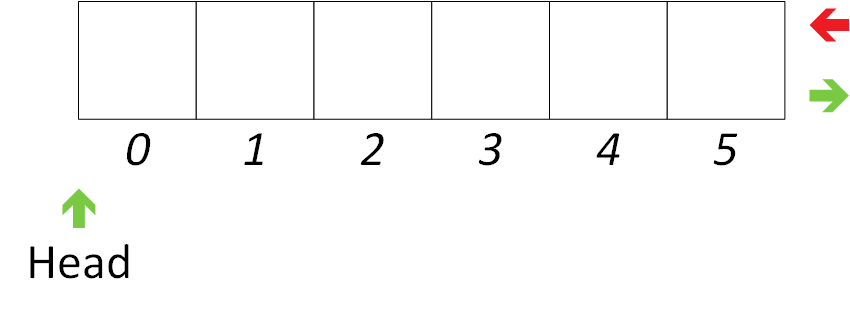
\includegraphics[scale=1]{img/piles/Piles_5_Tableau_Statique_Structure.png}
\end{center}

\smallskip

On notera cette fois que plusieurs informations distinctes doivent être conservées : l'adresse du tableau, le numéro de case correspondant au sommet de la pile (\textit{head} dans notre cas), la taille du tableau (le nombre maximum d'objets pouvant être stockés), le nombre d'éléments dans le tableau.

Le schéma suivant détaille certaines informations de façon plus explicite :\\

\begin{center}
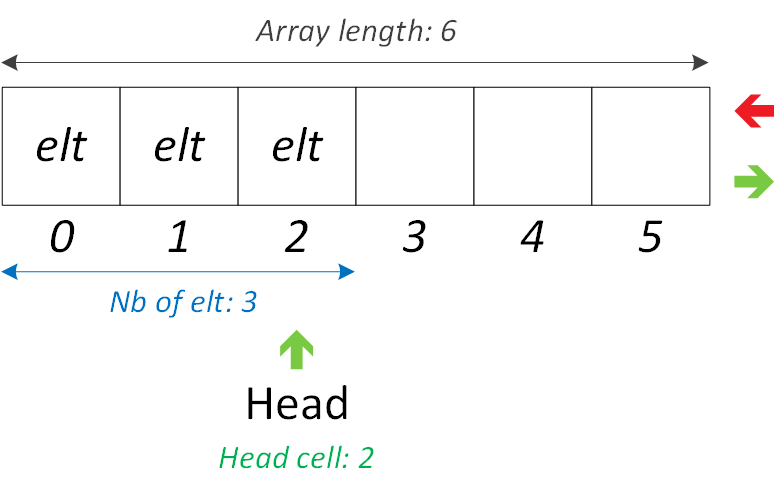
\includegraphics[scale=1]{img/piles/Piles_5_Tableau_Statique_Structure_Detaillee.png}
\end{center}

\smallskip

Dans le cas d'un tableau de taille fixe, le pointeur de sommet ne peut pas utiliser la valeur \TTBF{NULL} comme indicateur de tableau vide, car cette valeur est égale à $ 0 $ (ce qui laisserait à penser que le sommet est effectivement à la case 0).
Plusieurs solutions sont possibles pour indiquer le sommet de la pile et le cas vide :

\begin{itemize}
\item On enregistre dans la structure de la pile une variable servant à compter le nombre d'éléments présents (le sommet peut donc prendre n'importe quelle valeur tant que la pile est vide).
\item On utilise un entier relatif pour indiquer le sommet, et $ -1 $ indique que la pile est vide (l'ajout d'un élément décalera le sommet à $ 0 $, c'est-à-dire la case où sera l'élément).
\item On place le sommet de la pile sur la première case non utilisée, et l'accès au premier élément se fait donc en retirant $ 1 $ au pointeur de sommet (ainsi, un sommet à la case $ 0 $ indique que la pile est vide).
Attention : dans ce cas précis, un tableau plein aura un sommet hors des cases du tableau (il ne faudra donc \textit{jamais} le déréférencer s'il atteinte une telle valeur).
\end{itemize}

\smallskip

L'exemple suivant montre l'évolution d'une pile implémentée avec un tableau fixe au fur et à mesure des ajouts (empiler / \TTBF{PUSH}) et suppressions (dépiler / \TTBF{POP}).\\

\vfillFirst

\begin{center}
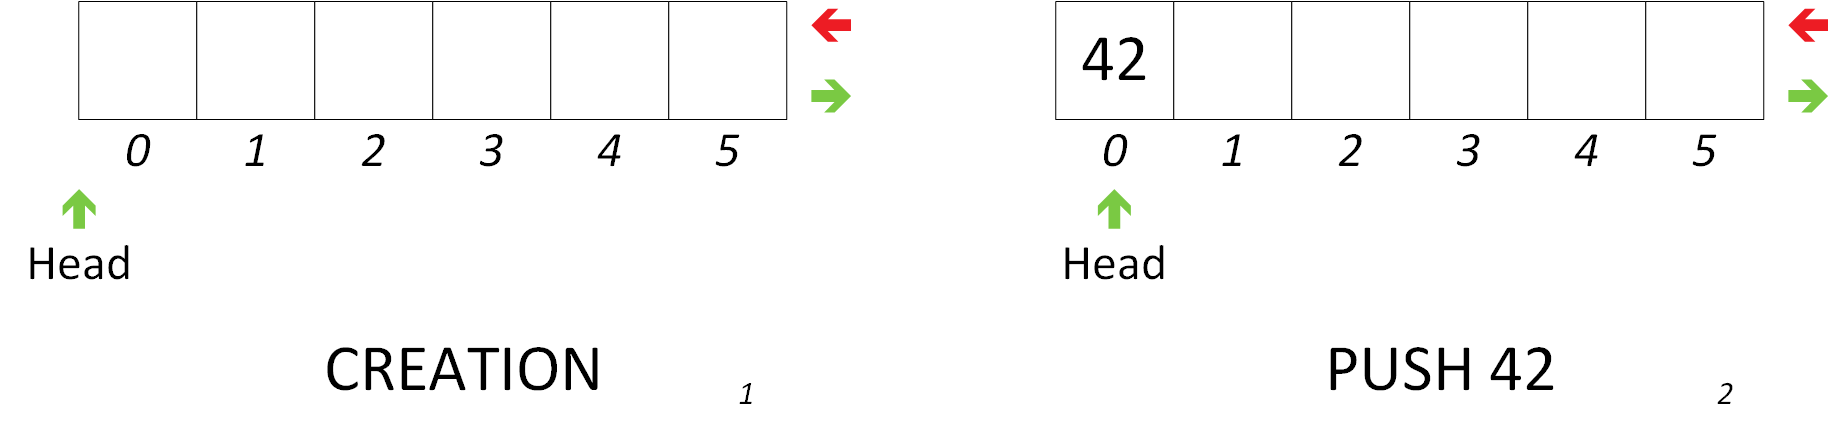
\includegraphics[scale=0.65]{img/piles/Piles_6_Tableau_Statique_Usage_pack_1.png}
\end{center}

\begin{center}
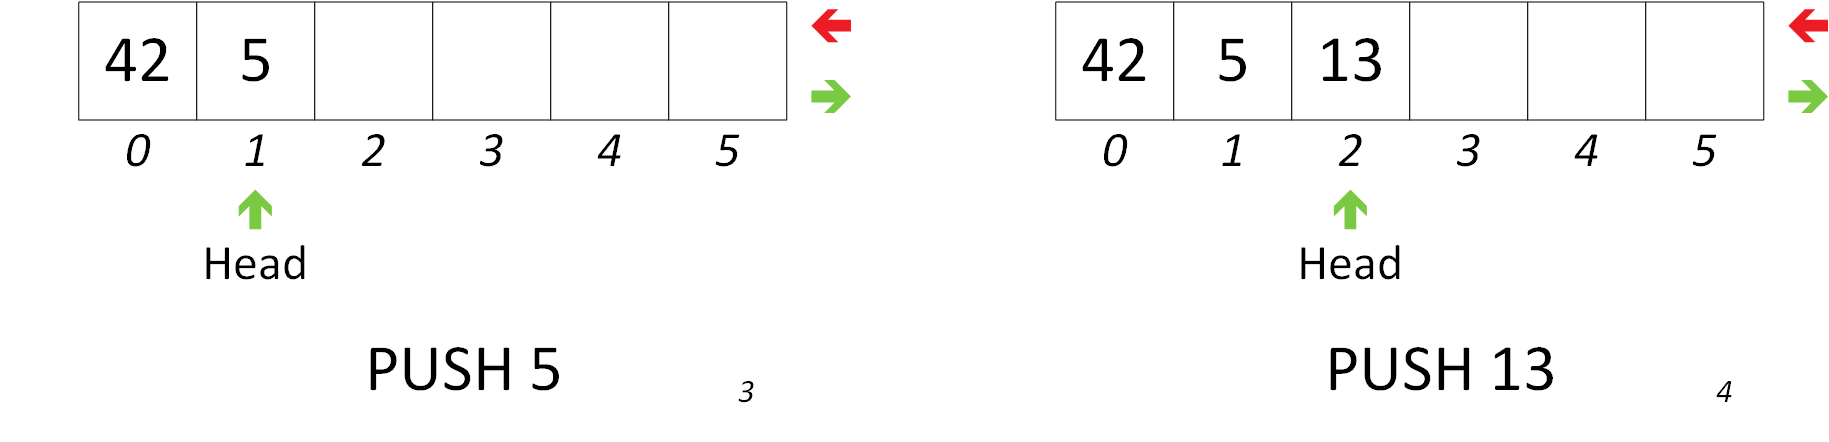
\includegraphics[scale=0.65]{img/piles/Piles_6_Tableau_Statique_Usage_pack_2.png}
\end{center}

\vfillLast

\pagebreak

\begin{center}
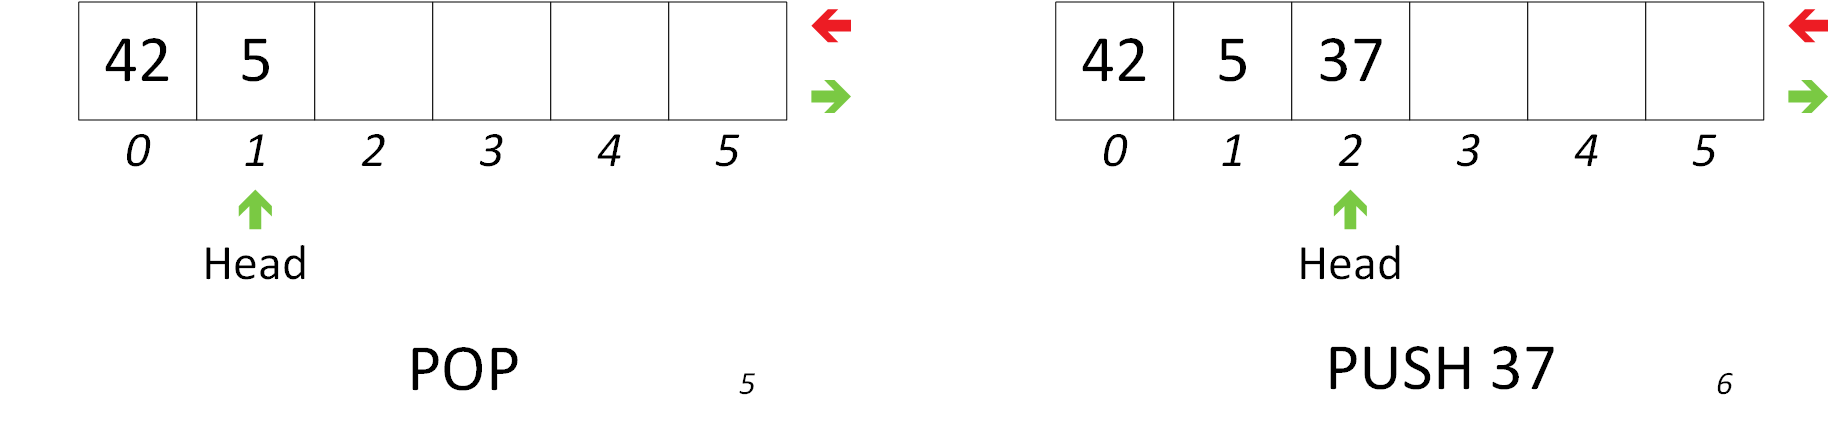
\includegraphics[scale=0.65]{img/piles/Piles_6_Tableau_Statique_Usage_pack_3.png}
\end{center}

\smallskip

Les principales opérations se résument ainsi :
\begin{itemize}
\item \TTBF{CreerPile() : Pile}\\
      La fonction alloue en mémoire le tableau (sauf s'il est statique), et elle fixe le sommet de la pile à la valeur prévue pour démarrer ($ -1 $, $ 0 $, ou toute autre valeur choisie). Éventuellement on met à jour le nombre d'objets dans le tableau en le fixant à $ 0 $
\item \TTBF{Empiler(Pile, Elt) : booléen}\\
      La fonction ajoute un élément au sommet de la pile s'il y a de la place et elle renvoie vrai, sinon, si la pile est pleine, elle renvoie faux sans rien faire d'autre
\item \TTBF{Dépiler(Pile) : booléen}\\
      La fonction supprime l'élément au sommet de la pile s'il y en a un et elle renvoie vrai, sinon, si la pile est vide, elle renvoie faux sans rien faire d'autre
\item \TTBF{Vider(Pile) : entier}\\
      La fonction fixe le sommet de la pile à la valeur prévue pour démarrer ($ -1 $, $ 0 $, ou toute autre valeur choisie). Elle renvoie le nombre d'éléments supprimés (c'est-à-dire combien ne sont plus référencés)
\item \TTBF{Sommet(Pile) : [Type Elt]}\\
      La fonction renvoie l'élément au sommet de la pile, ou s'il n'y en a pas, elle lève une exception, ou renvoie un pointeur \TTBF{NULL}, ou écrit un message d'erreur sans rien faire
\end{itemize}


\bigskip

%%%%%%%%%%%%%%%%%%%

\subsection{Piles avec pointeurs}

\bigskip

Une implémentation à l'aide d'une liste chaînée permet d'exploiter la mémoire et d'être donc beaucoup plus flexible en terme de nombre maximum d'éléments.
Le schéma suivant illustre une pile sous forme de liste chaînée en mémoire :\\

\begin{center}
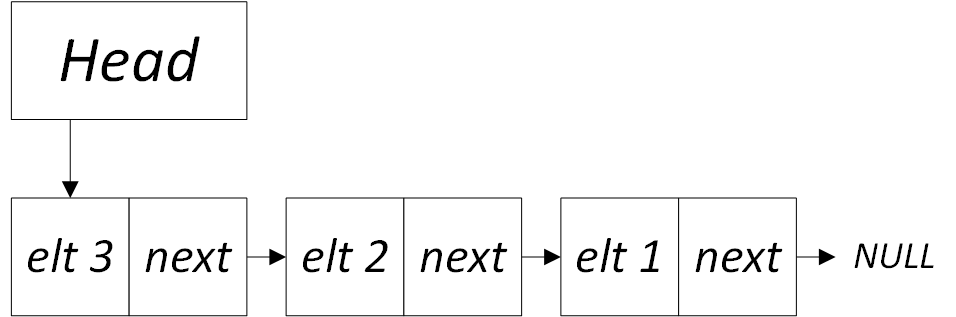
\includegraphics[scale=0.75]{img/piles/Piles_3_Liste_Chainee_Structure_cas_general.png}
\end{center}

\smallskip

On y retrouve plusieurs fois la structure typique des listes chaînées (un élément et un pointeur vers l'élément suivant), ainsi qu'un pointeur indiquant le sommet de la pile (\textit{head} dans notre cas).

L'unique cas particulier concerne une pile vide : le pointeur de sommet vaut dans ce cas \TTBF{NULL}.
Il s'agit également de l'état dans lequel se trouve une pile vidée ou nouvellement créée.\\

\begin{center}
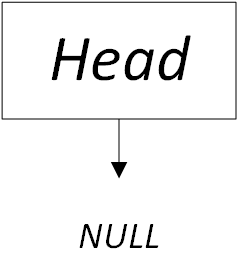
\includegraphics[scale=0.75]{img/piles/Piles_3_Liste_Chainee_Structure_cas_vide.png}
\end{center}

\smallskip

L'exemple suivant montre l'évolution d'une pile au fur et à mesure des ajouts (empiler / \TTBF{PUSH}) et suppressions (dépiler / \TTBF{POP}).\\

\begin{center}
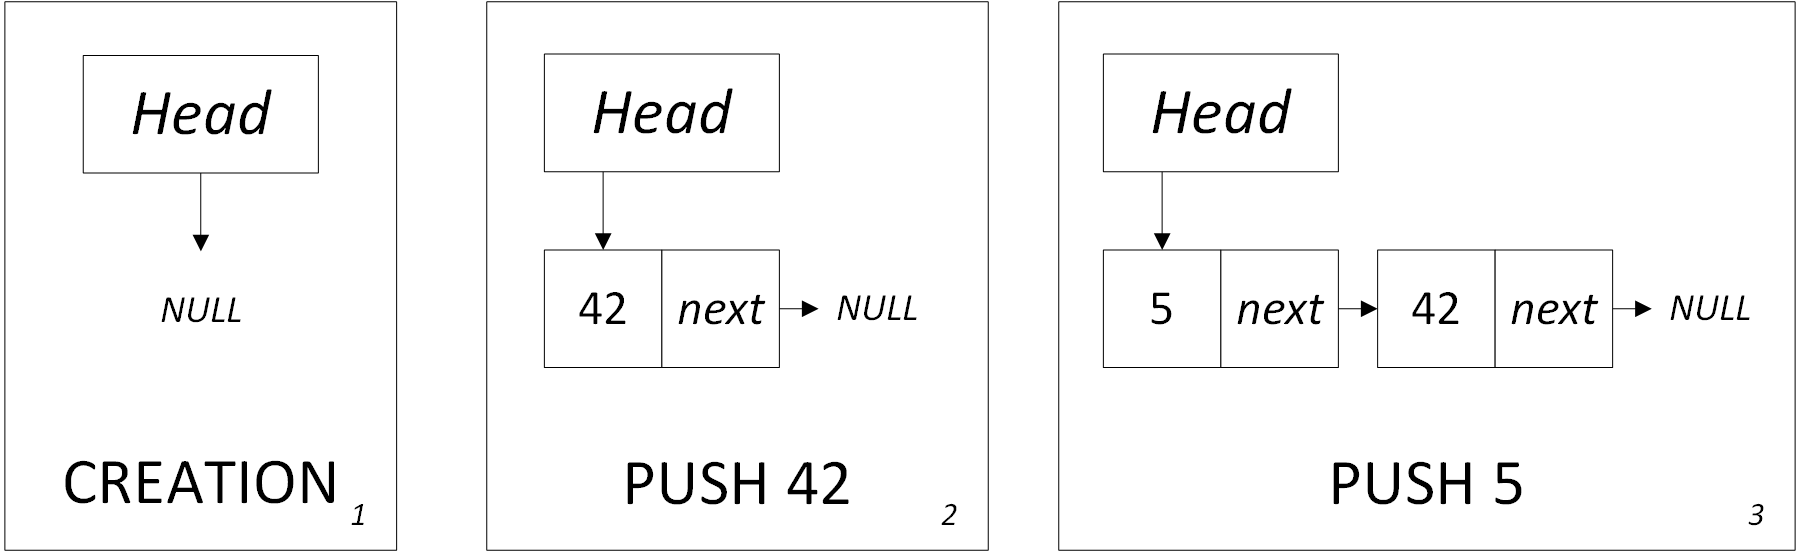
\includegraphics[scale=0.65]{img/piles/Piles_4_Liste_Chainee_Usage_pack_1.png}
\end{center}

\begin{center}
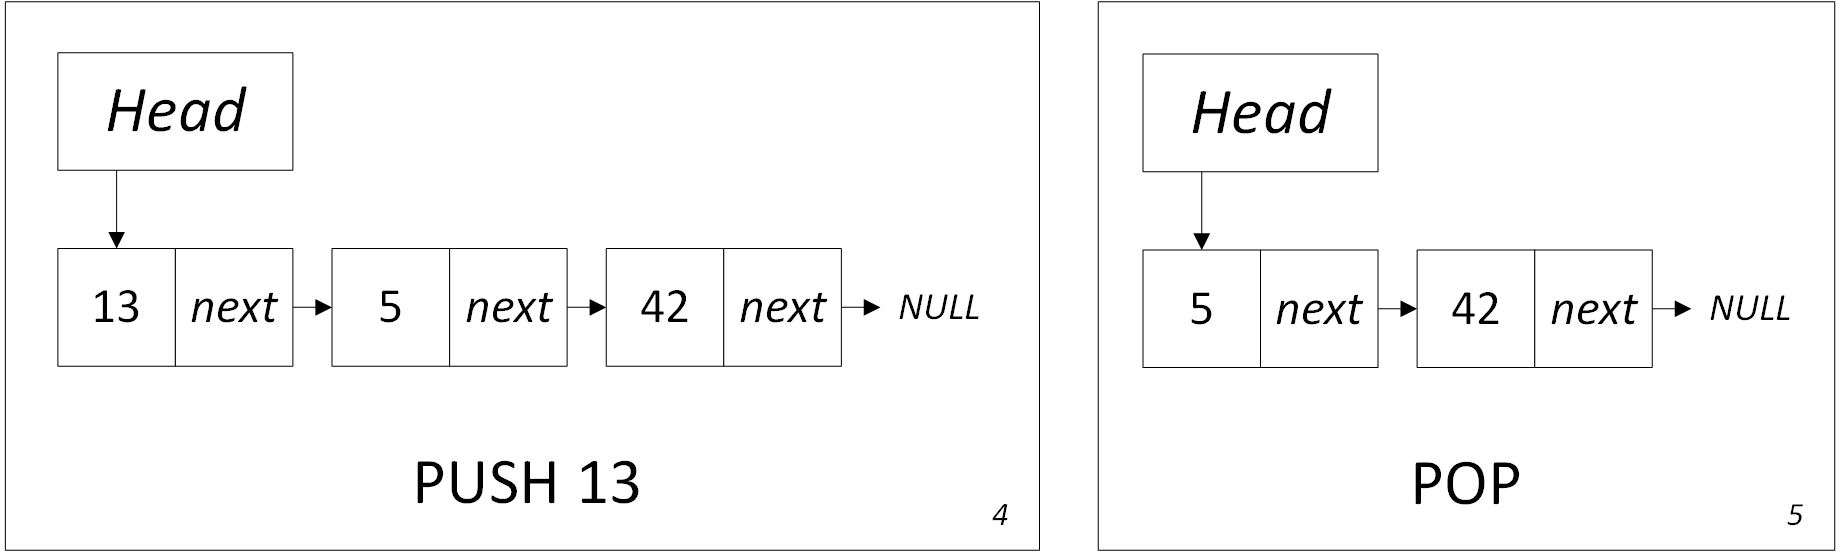
\includegraphics[scale=0.65]{img/piles/Piles_4_Liste_Chainee_Usage_pack_2.png}
\end{center}

\smallskip

Les principales opérations se résument ainsi :
\begin{itemize}
\item \TTBF{CreerPile() : Pile}\\
      La fonction alloue en mémoire la structure générale de la pile, et elle fixe le sommet de la pile à \TTBF{NULL}
\item \TTBF{Empiler(Pile, Elt) : booléen}\\
      La fonction alloue en mémoire un nouvel élément dont le pointeur \textit{next} pointe vers l'actuel élément au sommet de la pile, puis, elle met à jour le pointeur de sommet de la pile vers l'adresse de ce nouvel élément
\item \TTBF{Dépiler(Pile) : booléen}\\
      La fonction retourne une erreur si la pile est vide, sinon, elle récupère tout d'abord l'adresse de l'élément suivant celui au sommet, puis, elle libère l'élément au sommet, puis, elle met à jour le pointeur de sommet de la pile vers l'adresse de l'élément suivant
\item \TTBF{Vider(Pile) : entier}\\
      La fonction dépile successivement tous les éléments jusqu'à obtenir un sommet à \TTBF{NULL}
\item \TTBF{Sommet(Pile) : [Type Elt]}\\
      La fonction renvoie l'élément au sommet de la pile, ou s'il n'y en a pas, elle lève une exception, ou renvoie un pointeur \TTBF{NULL}, ou écrit un message d'erreur sans rien faire
\item \TTBF{Supprimer(Pile)}\\
      La fonction supprime la structure générale de la pile en mémoire, éventuellement en la vidant juste avant
\end{itemize}


\newpage

%%%%%%%%%%%%%%%%%%%%%%%%%%%%%%%%%%%%%%

\section{Files}

\bigskip

Les \textbf{files}, ou \textbf{queues} en anglais, sont des structures visant à stocker et rendre les données dans l'ordre d'arrivée.
Une file dispose donc d'une \textit{tête} contenant l'élément le plus ancien (inséré avant tous les autres), et une \textit{queue} contenant l'élément inséré le plus récemment.
Ces structures sont aussi appelées \textbf{FIFO} (\textit{First In First Out}).\\

\begin{center}
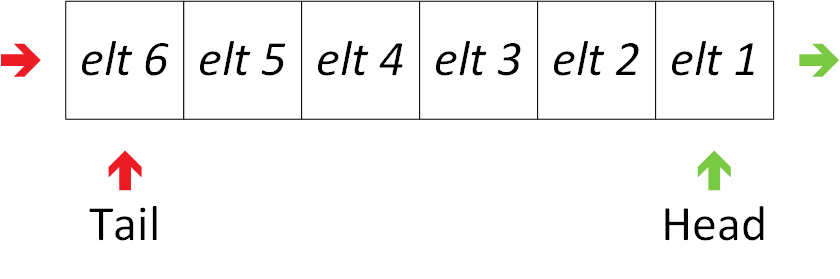
\includegraphics[scale=0.75]{img/files/Files_1_Structure_Generale.png}
\end{center}

\smallskip

Deux opérations permettent d'utiliser une file :
\begin{itemize}
\item \TTBF{ENQUEUE} : permettant d'\textit{enfiler} une donnée supplémentaire dans la file
\item \TTBF{DEQUEUE} : permettant de \textit{défiler} une donnée depuis la file
\end{itemize}
On ajoute donc une donnée en l'enfilant avec un \TTBF{ENQUEUE}, celle-ci se retrouve en \textit{queue} de file, c'est-à-dire au fond de la file.
On récupère une donnée en défilant avec un \TTBF{DEQUEUE}, celle-ci se trouvait en \textit{tête} de file, c'est-à-dire qu'elle attendait son tour depuis son insertion.
On accède donc aux éléments dans l'ordre d'arrivée.\\

Voici un exemple où l'on crée une file, puis on enfile successivement $ 42 $, $ 5 $, et $ 13 $, puis, on défile une fois (pour récupérer $ 42 $), et enfin, on enfile successivement $ 37 $, $ 10 $, $ 24 $, et $ 8 $.\\

\begin{center}
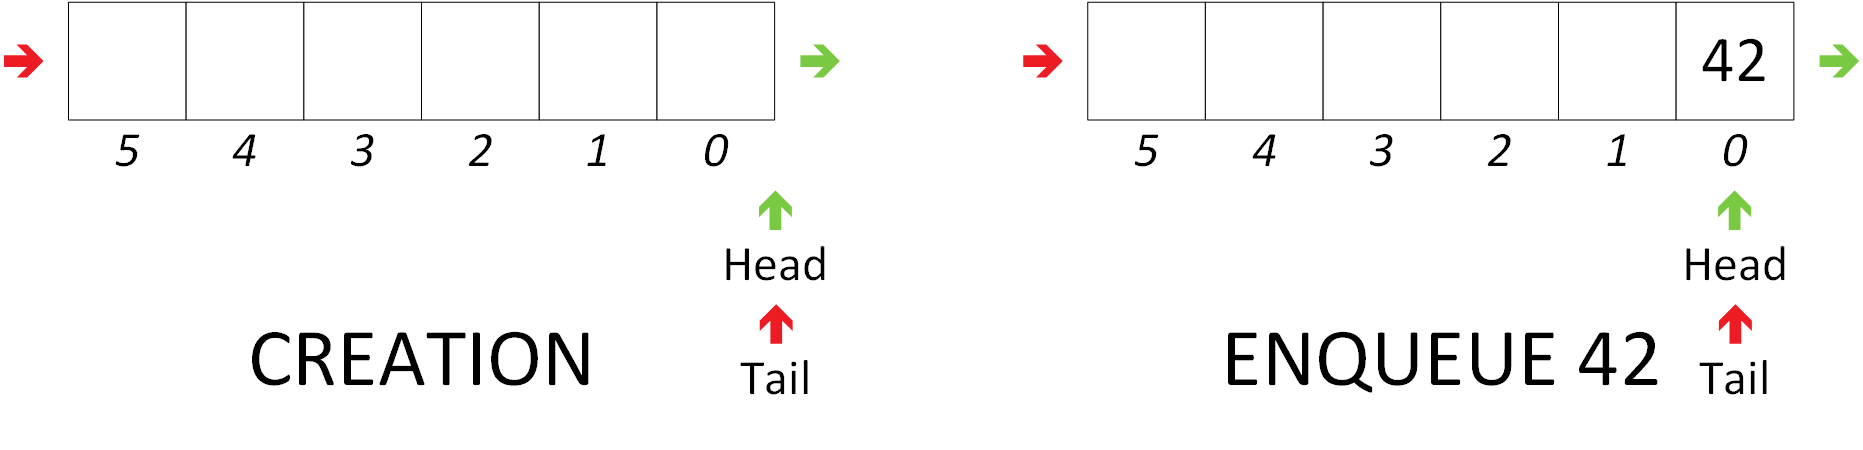
\includegraphics[scale=0.65]{img/files/Files_2_Structure_Generale_Usage_pack_1.png}
\end{center}

\begin{center}
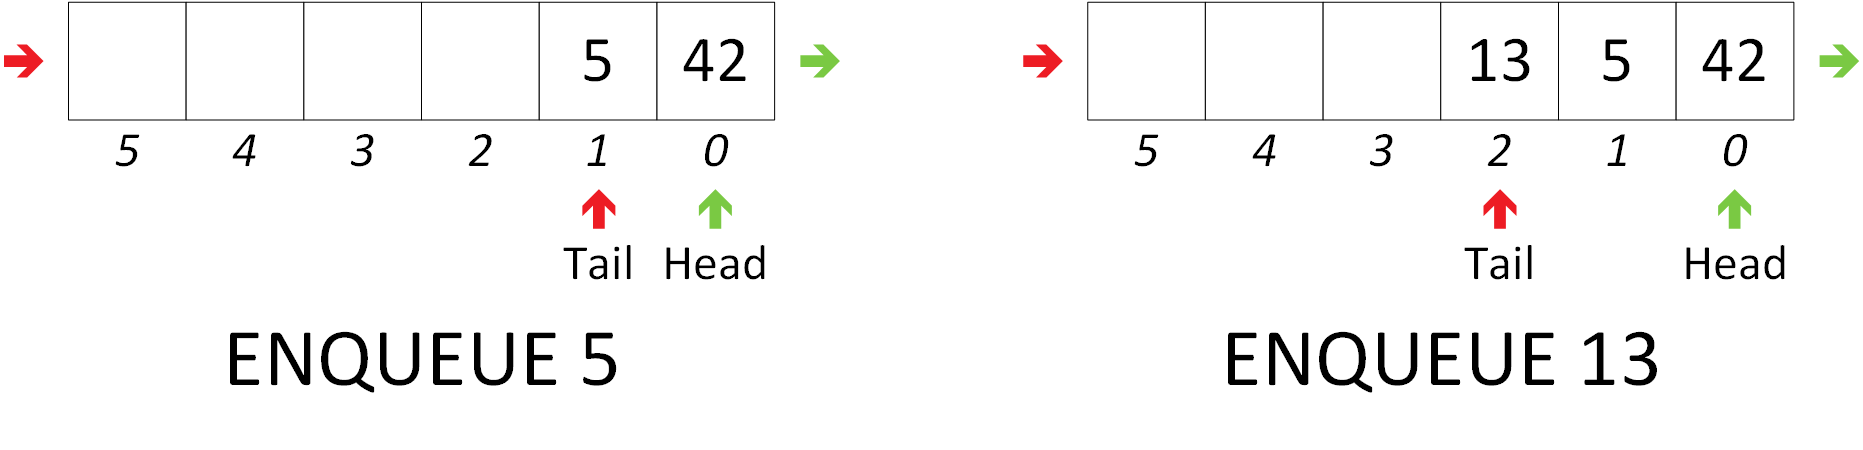
\includegraphics[scale=0.65]{img/files/Files_2_Structure_Generale_Usage_pack_2.png}
\end{center}

\begin{center}
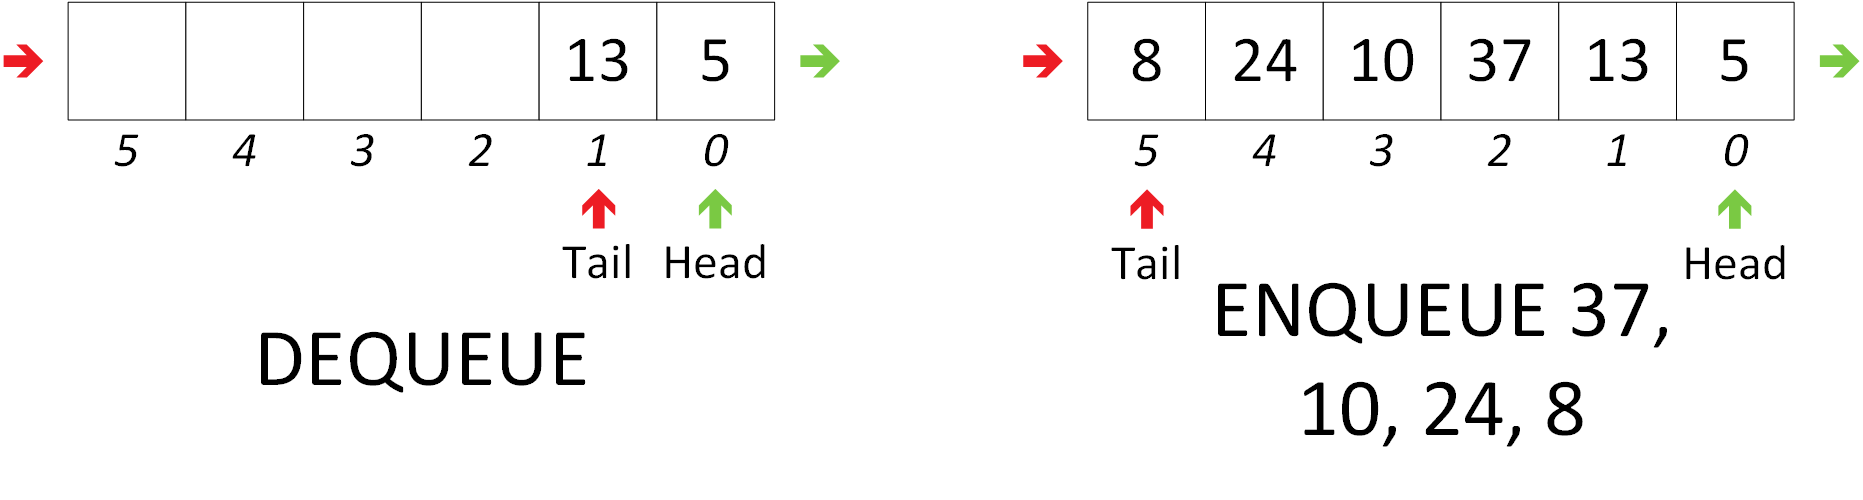
\includegraphics[scale=0.65]{img/files/Files_2_Structure_Generale_Usage_pack_3.png}
\end{center}

\smallskip

Les files, et surtout le respect de l'ordre d'arrivée des objets, sont couramment utilisés : mise en attente de personnes face à des guichets (voitures à un péage, clients face à une caisse, etc).

En informatique, on utilisera les files pour stocker temporairement et traiter les requêtes dans leur ordre d'arrivée.
Dans le cas des \textit{schedulers} (ordonnanceurs) visant à déterminer quel processus exécuter sur le c\oe{}ur d'un processus, on ajoute parfois une priorité à chaque objet de la file.
Ceci implique de mettre à jour l'ordre des objets dans la file lors de certains évènements (par exemple lorsque l'on enfile ou défile un élément, ou après un certain temps).\\

Afin d'implémenter une file, il est donc nécessaire d'avoir un espace de stockage ordonné (un tableau numéroté ou une liste chaînée), et deux indicateurs pour l'élément tête de file et l'élément en queue de file.
Nous allons maintenant voir comment implémenter une file avec des listes chaînées et un tableau de taille fixe.


\bigskip

%%%%%%%%%%%%%%%%%%%

\subsection{Files avec tableaux}

\bigskip

Une implémentation avec un tableau de taille fixe impose cette fois une limitation : la file aura une taille maximale, et on peut refuser l'ajout d'un élément si la file est déjà pleine.
La structure diffère également du fait que le tableau est alloué une seule fois lors de sa création (voire même lors de la compilation dans le cas statique).

Le schéma suivant présente la structure générale :\\

\begin{center}
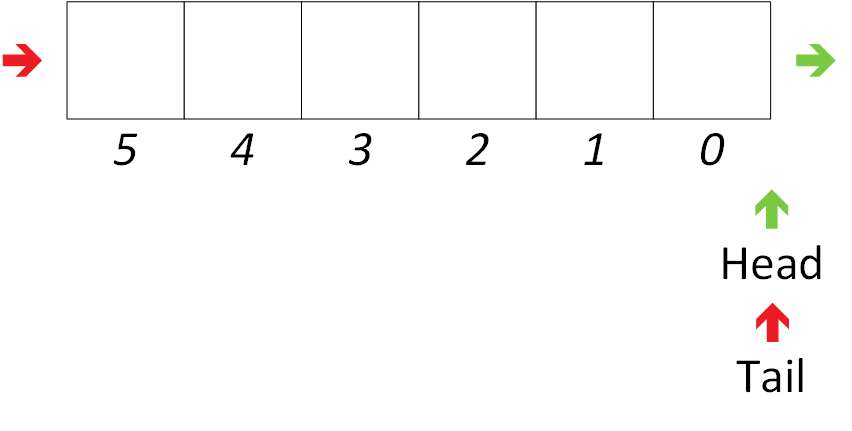
\includegraphics[scale=1]{img/files/Files_5_Tableau_Statique_Structure.png}
\end{center}

\smallskip

On notera cette fois que plusieurs informations distinctes doivent être conservées : l'adresse du tableau, le numéro de case correspondant à la tête de la file (\textit{head}), le numéro de case correspondant à la queue de la file (\textit{tail}), la taille du tableau (le nombre maximum d'objets pouvant être stockés), le nombre d'éléments dans le tableau.

Le schéma suivant détaille certaines informations de façon plus explicite :\\

\begin{center}
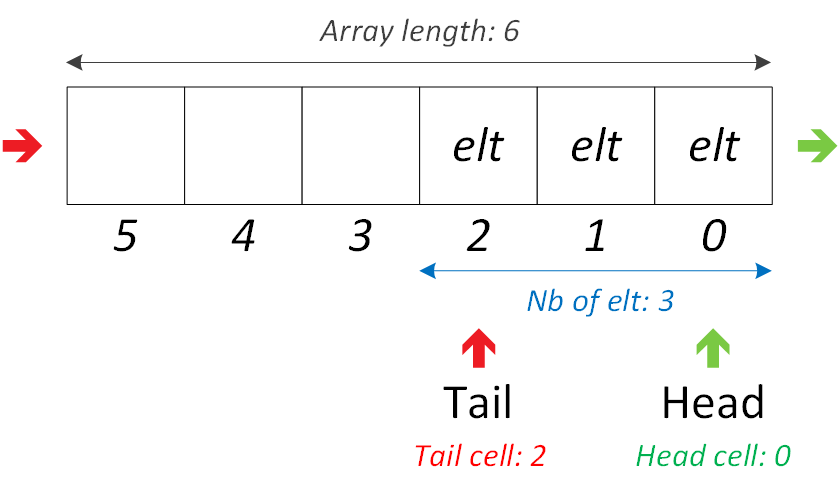
\includegraphics[scale=1]{img/files/Files_5_Tableau_Statique_Structure_Detaillee_1.png}
\end{center}

\smallskip

Une façon d'implémenter le tableau permet de supposer que la case $ 0 $ contiendra toujours l'élément de tête.
Dans ce cas très précis, on peut donc se passer de la variable de tête, et au contraire, s'appuyer sur la variable donnant le nombre d'éléments dans le tableau pour savoir si la file est vide ou non.
Cette implémentation ressemble donc à cela :\\

\begin{center}
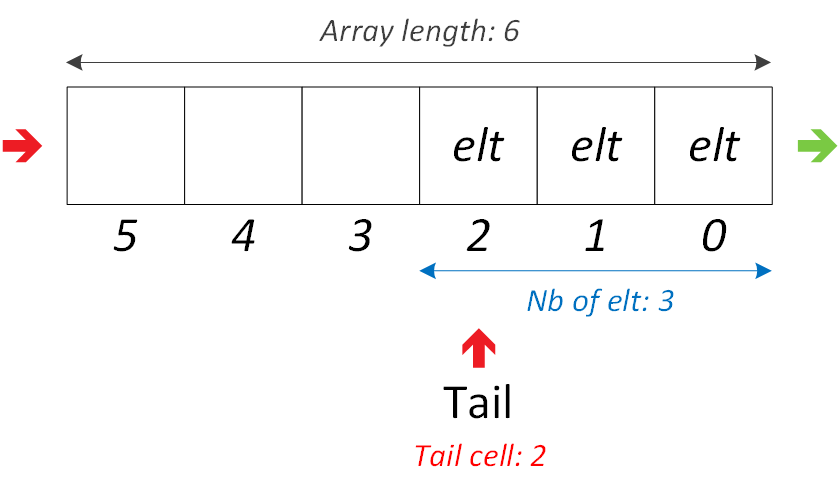
\includegraphics[scale=1]{img/files/Files_5_Tableau_Statique_Structure_Detaillee_2.png}
\end{center}

\smallskip

Dans le cas d'un tableau de taille fixe, les pointeurs de tête et de queue ne peuvent pas utiliser la valeur \TTBF{NULL} comme indicateur de tableau vide, car cette valeur est égale à $ 0 $ (ce qui laisserait à penser que la queue est effectivement à la case 0).
Plusieurs solutions sont possibles pour indiquer les cases où se trouvent la tête et la queue de la file, ainsi que le cas vide :

\begin{itemize}
\item On enregistre dans la structure de la file une variable servant à compter le nombre d'éléments présents (la queue peut donc prendre n'importe quelle valeur tant que la file est vide).
\item On utilise un entier relatif pour indiquer la position, et $ -1 $ indique que la file est vide (l'ajout d'un élément décalera la tête et la queue à $ 0 $, c'est-à-dire la case où sera l'élément).
\item On place la queue de la file sur la première case non utilisée, et l'accès au dernier élément se fait donc en retirant $ 1 $ au pointeur de sommet (ainsi, une queue à la case $ 0 $ indique que la file est vide).
Attention : dans ce cas précis, un tableau plein aura un sommet hors des cases du tableau (il ne faudra donc \textit{jamais} le déréférencer s'il atteinte une telle valeur).
\item On représente complètement différemment la file : on décale les pointeurs de tête et de queue au fur et à mesure des insertions et suppressions ($ +1 $ / $ -1 $). Le pointeur de queue peut passer de la dernière case à la première, car les éléments actuellement dans la file se trouvent uniquement entre la tête et la queue.
Vider ce tableau revient uniquement à passer les pointeurs à la valeur $ -1 $.
Attention : dans ce cas précis, il est nécessaire de faire très attention à l'ordre de lecture des éléments entre la tête et la queue.
\end{itemize}

\smallskip

L'exemple suivant montre l'évolution d'une file implémentée avec un tableau fixe au fur et à mesure des ajouts (enfiler / \TTBF{ENQUEUE}) et suppressions (défiler / \TTBF{DEQUEUE}).\\

\begin{center}
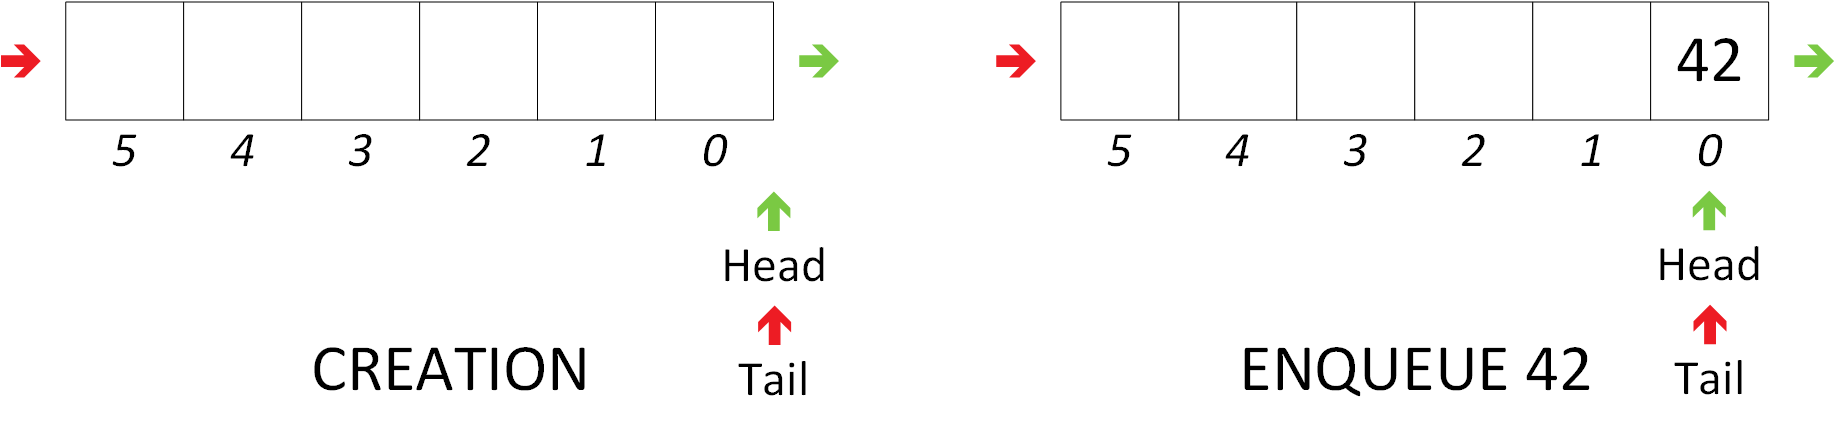
\includegraphics[scale=0.65]{img/files/Files_6_Tableau_Statique_Usage_pack_1.png}
\end{center}

\begin{center}
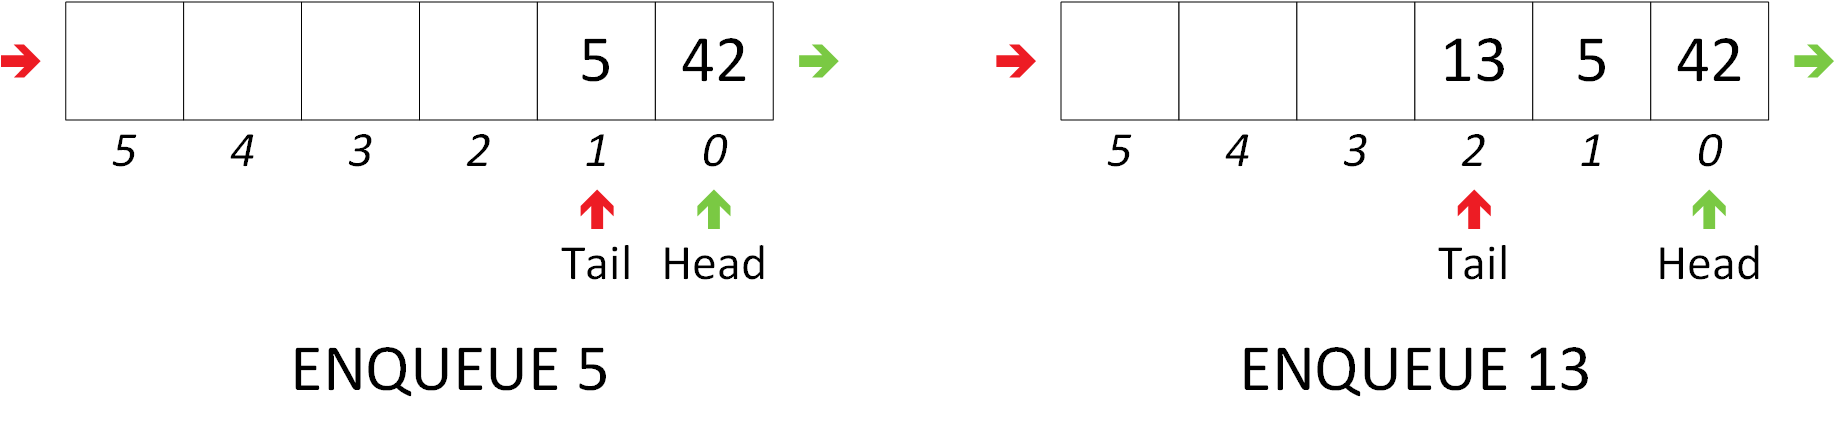
\includegraphics[scale=0.65]{img/files/Files_6_Tableau_Statique_Usage_pack_2.png}
\end{center}

\smallskip

Dans les schémas suivants, deux versions sont présentées :
\begin{itemize}
\item celui de gauche présente la version standard où la tête ne bouge pas (il est nécessaire de décaler l'ensemble des éléments du tableau dès que l'on défile),
\item celui de droite présente la version où seuls les pointeurs de tête et de queue sont décalés (il faut faire attention à l'ordre de lecture entre la tête et la file, et s'appuyer sur les modulos).
\end{itemize}

\begin{center}
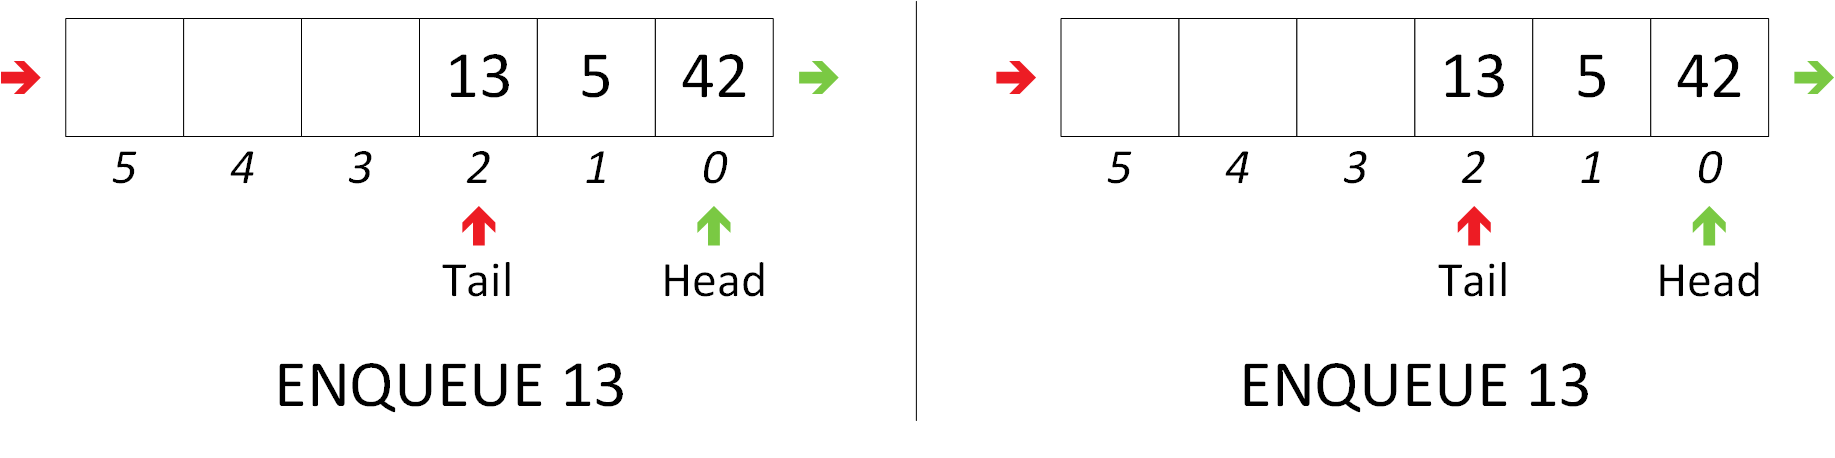
\includegraphics[scale=0.65]{img/files/Files_6_Tableau_Statique_Usage_pack_2_double.png}
\end{center}

\begin{center}
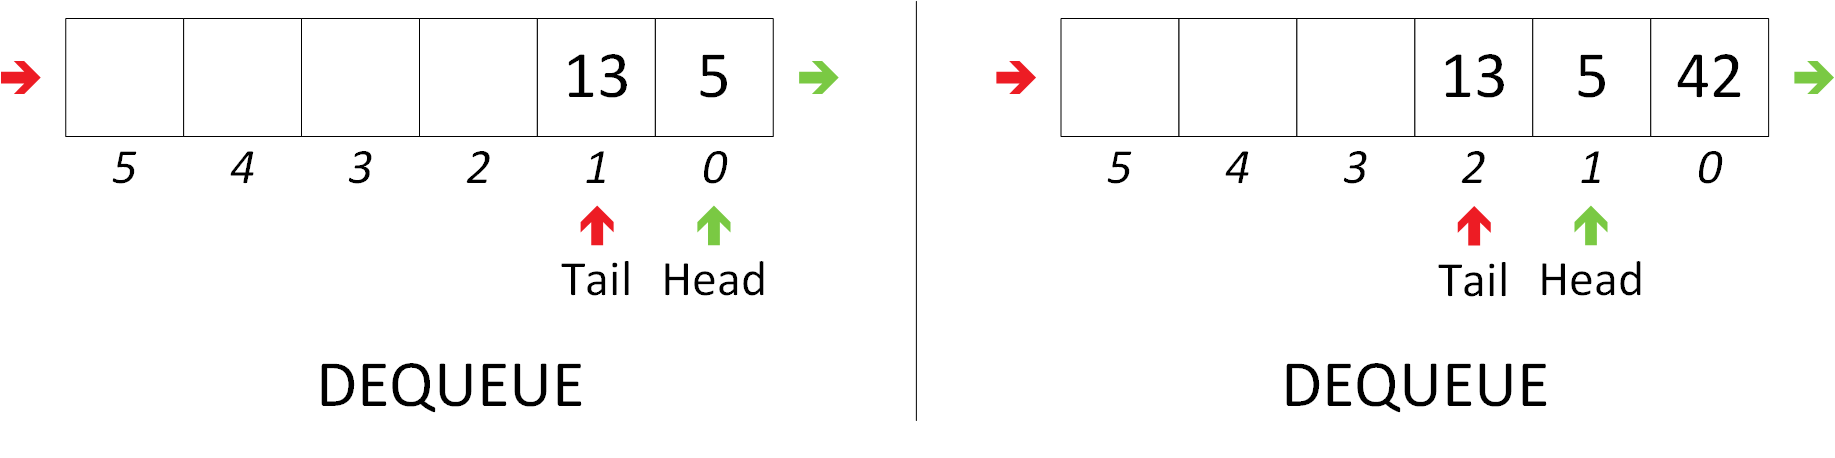
\includegraphics[scale=0.65]{img/files/Files_6_Tableau_Statique_Usage_pack_3.png}
\end{center}

\begin{center}
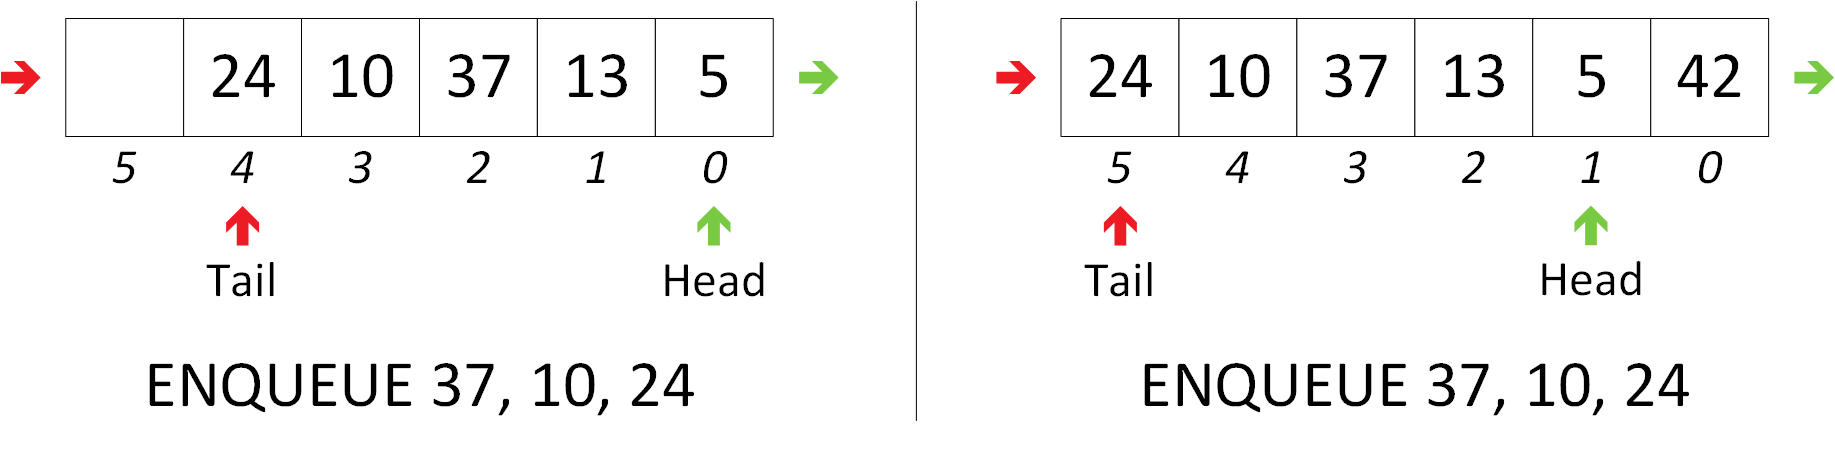
\includegraphics[scale=0.65]{img/files/Files_6_Tableau_Statique_Usage_pack_4.png}
\end{center}

\begin{center}
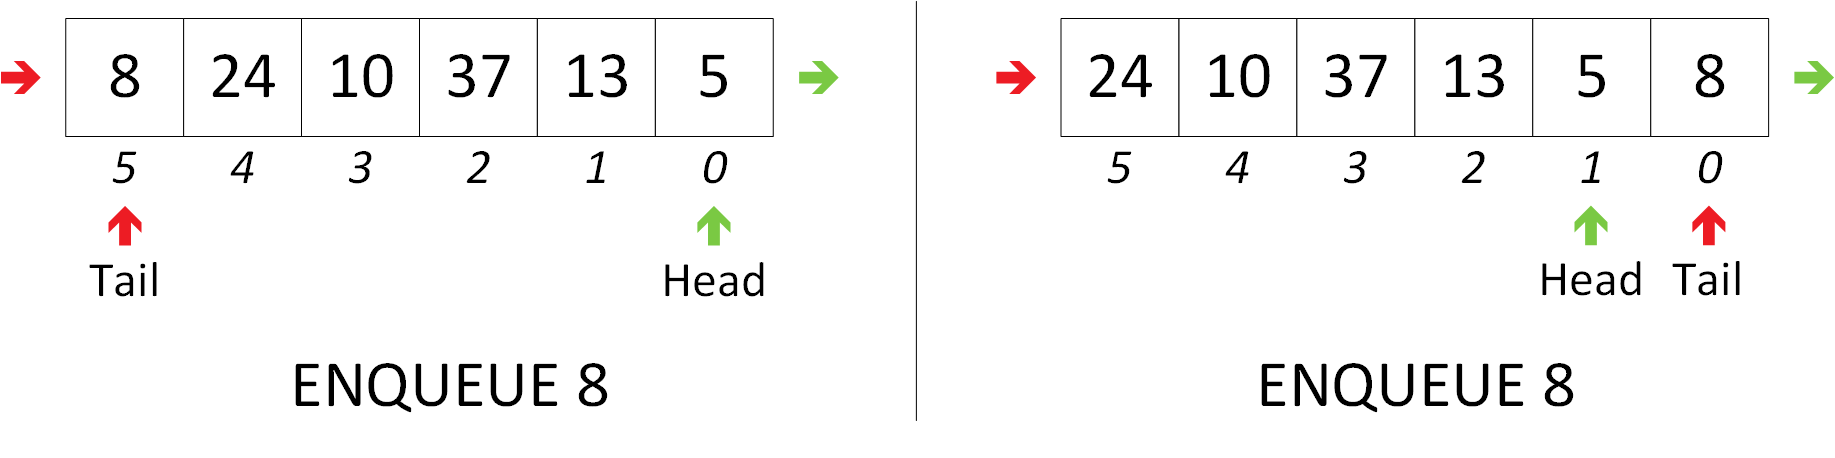
\includegraphics[scale=0.65]{img/files/Files_6_Tableau_Statique_Usage_pack_5.png}
\end{center}

\smallskip

Dans ce dernier cas, lorsque le tableau de gauche était complètement rempli, on a décalé le pointeur de queue au début du tableau, simplement en utilisant un modulo de la taille du tableau.
Il est important de respecter l'ordre de lecture : on lit bel et bien depuis le pointeur de tête, en effectuant un $ +1 $ (lecture vers la gauche) tout en appliquant un modulo de la taille du tableau au résultat, jusqu'à atteindre le pointeur de queue.

On peut également comprendre qu'il y a eu un dépassement en comparant la position du pointeur de tête et de queue : la différence entre leurs positions est négative ! \linebreak
($ pos. tail - pos. head = 0 - 1 = -1$)

\bigskip

Cette autre façon de gérer la file est un tout petit peu plus complexe dans l'écriture des algorithmes de gestion, mais elle évite énormément de réécritures dans le tableau/en mémoire (inutile de lire une case, l'écrire ailleurs, et recommencer ainsi de suite lors de chaque \textit{dequeue}).
Pour ce TP, vous êtes libres de choisir l'implémentation que vous souhaitez réaliser.

\bigskip

Les principales opérations se résument ainsi :
\begin{itemize}
\item \TTBF{CreerFile() : File}\\
      La fonction alloue en mémoire le tableau (sauf s'il est statique), et elle fixe la tête et la queue de la file à la valeur prévue pour démarrer ($ -1 $, $ 0 $, ou toute autre valeur choisie). Éventuellement on met à jour le nombre d'objets dans le tableau en le fixant à $ 0 $
\item \TTBF{Enfiler(File, Elt) : booléen}\\
      La fonction ajoute un élément en queue de file s'il y a de la place et met à jour la position de la queue, puis elle renvoie vrai, sinon, si la file est pleine, elle renvoie faux sans rien faire d'autre
\item \TTBF{Défiler(File) : booléen}\\
      La fonction supprime l'élément en tête de file s'il y en a un et décale tous les éléments d'un cran, puis elle renvoie vrai, sinon, si la file est vide, elle renvoie faux sans rien faire d'autre
\item \TTBF{Vider(File) : entier}\\
      La fonction fixe la tête et la queue à la valeur prévue pour démarrer ($ -1 $, $ 0 $, ou toute autre valeur choisie). Elle renvoie le nombre d'éléments supprimés (c'est-à-dire combien ne sont plus référencés)
\item \TTBF{Tête(File) : [Type Elt]}\\
      La fonction renvoie l'élément en tête de file (le prochain élément qui sera défilé), ou s'il n'y en a pas, elle lève une exception, ou renvoie un pointeur \TTBF{NULL}, ou écrit un message d'erreur sans rien faire
\item \TTBF{Queue(File) : [Type Elt]}\\
      La fonction renvoie l'élément en queue de file (le dernier élément qui sera défilé), ou s'il n'y en a pas, elle lève une exception, ou renvoie un pointeur \TTBF{NULL}, ou écrit un message d'erreur sans rien faire
\end{itemize}


\bigskip

%%%%%%%%%%%%%%%%%%%

\subsection{Files avec pointeurs}

\bigskip

Une implémentation à l'aide d'une liste chaînée permet d'exploiter la mémoire et d'être donc beaucoup plus flexible en terme de nombre maximum d'éléments.
Le schéma suivant illustre une file sous forme de liste chaînée en mémoire :\\

\begin{center}
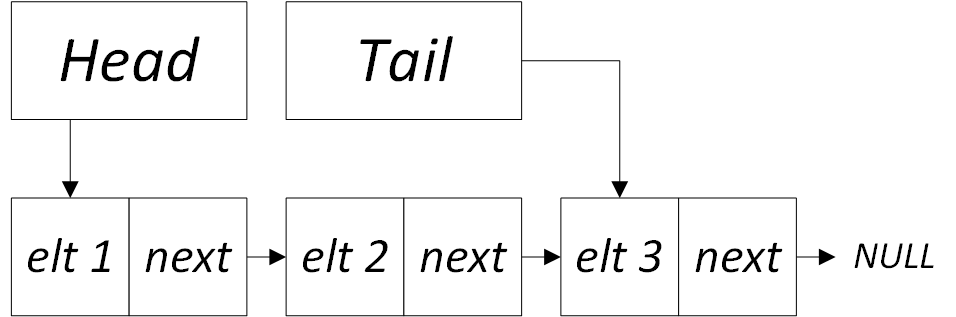
\includegraphics[scale=0.75]{img/files/Files_3_Liste_Chainee_Structure_cas_general.png}
\end{center}

\smallskip

On y retrouve plusieurs fois la structure typique des listes chaînées (un élément et un pointeur vers l'élément suivant), ainsi que deux pointeurs indiquant respectivement la tête de la file (\textit{head}) et la queue de la file (\textit{tail}).

Deux cas particuliers concernent les files où le pointeur de tête et le pointeur de queue valent la même chose : la file vide où les pointeurs contiennent \TTBF{NULL}, et la file contenant un seul élément vers lequel les deux pointeurs renvoient.
Une file nouvellement créée se trouve dans l'état vide.\\

\begin{center}
%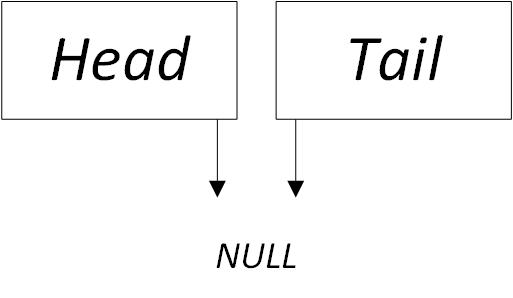
\includegraphics[scale=0.75]{img/files/Files_3_Liste_Chainee_Structure_cas_vide.png}
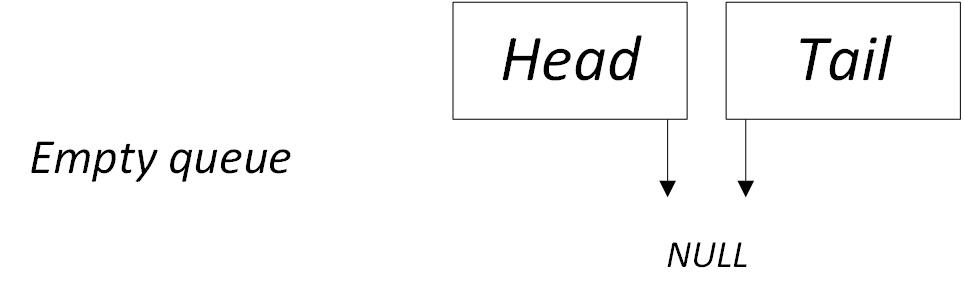
\includegraphics[scale=0.75]{img/files/Files_3_Liste_Chainee_Structure_cas_vide_etiquette.png}
\end{center}

\smallskip

\begin{center}
%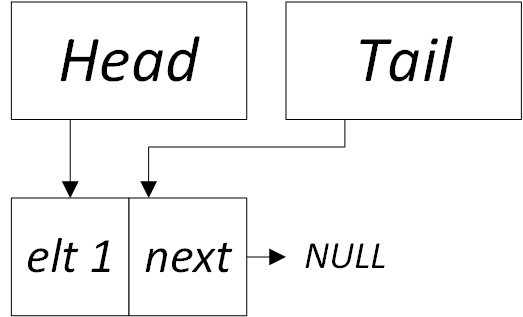
\includegraphics[scale=0.75]{img/files/Files_3_Liste_Chainee_Structure_cas_1_elt.png}
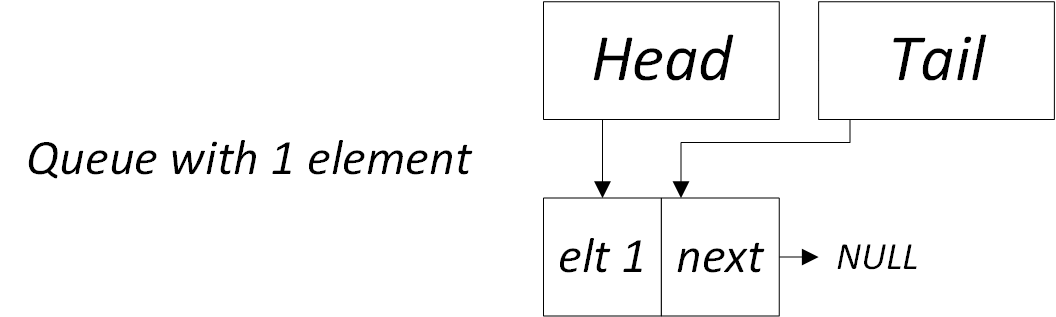
\includegraphics[scale=0.75]{img/files/Files_3_Liste_Chainee_Structure_cas_1_elt_etiquette.png}
\end{center}

\smallskip

L'exemple suivant montre l'évolution d'une file au fur et à mesure des insertions (enfiler / \TTBF{ENQUEUE}) et suppressions (défiler / \TTBF{DEQUEUE}).\\

\begin{center}
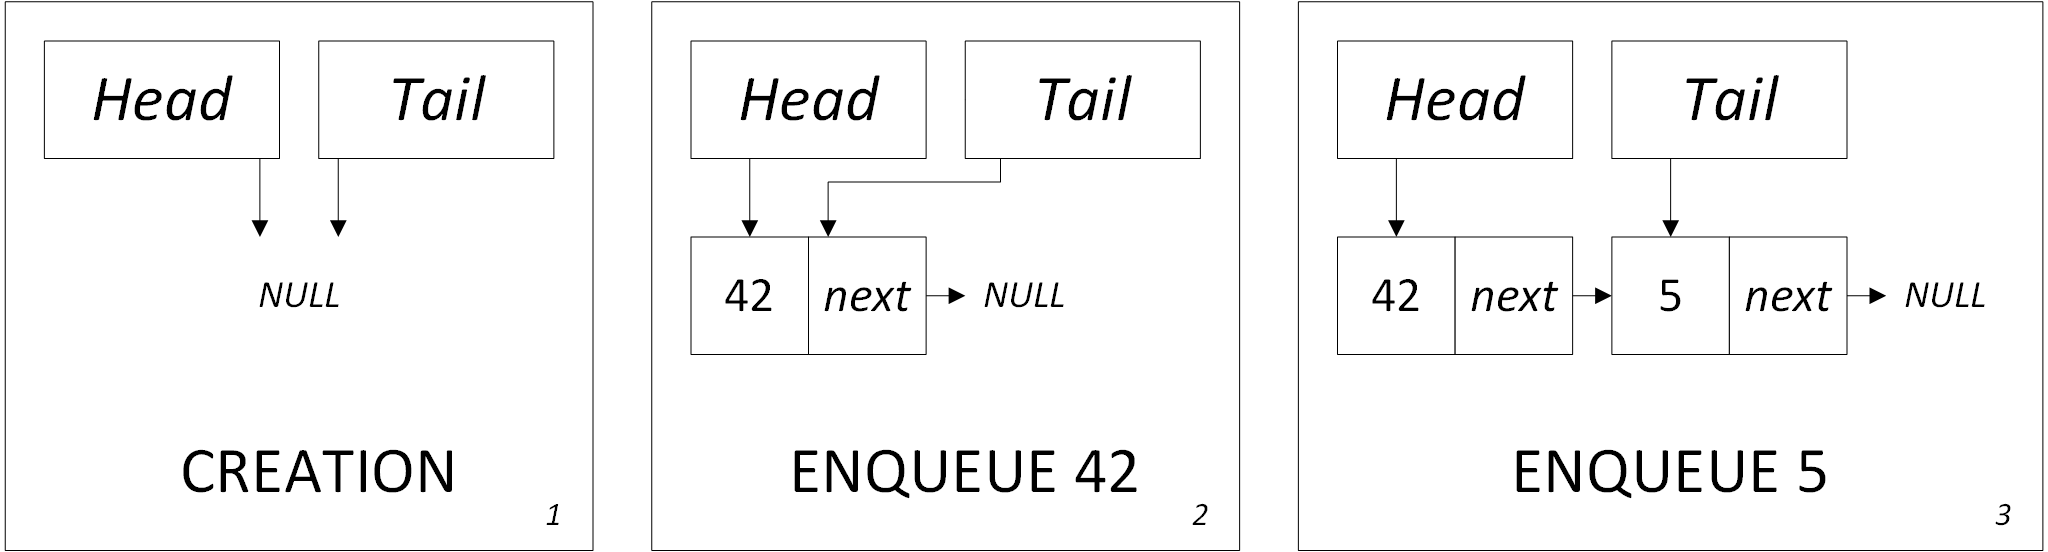
\includegraphics[scale=0.60]{img/files/Files_4_Liste_Chainee_Usage_pack_1.png}
\end{center}

\begin{center}
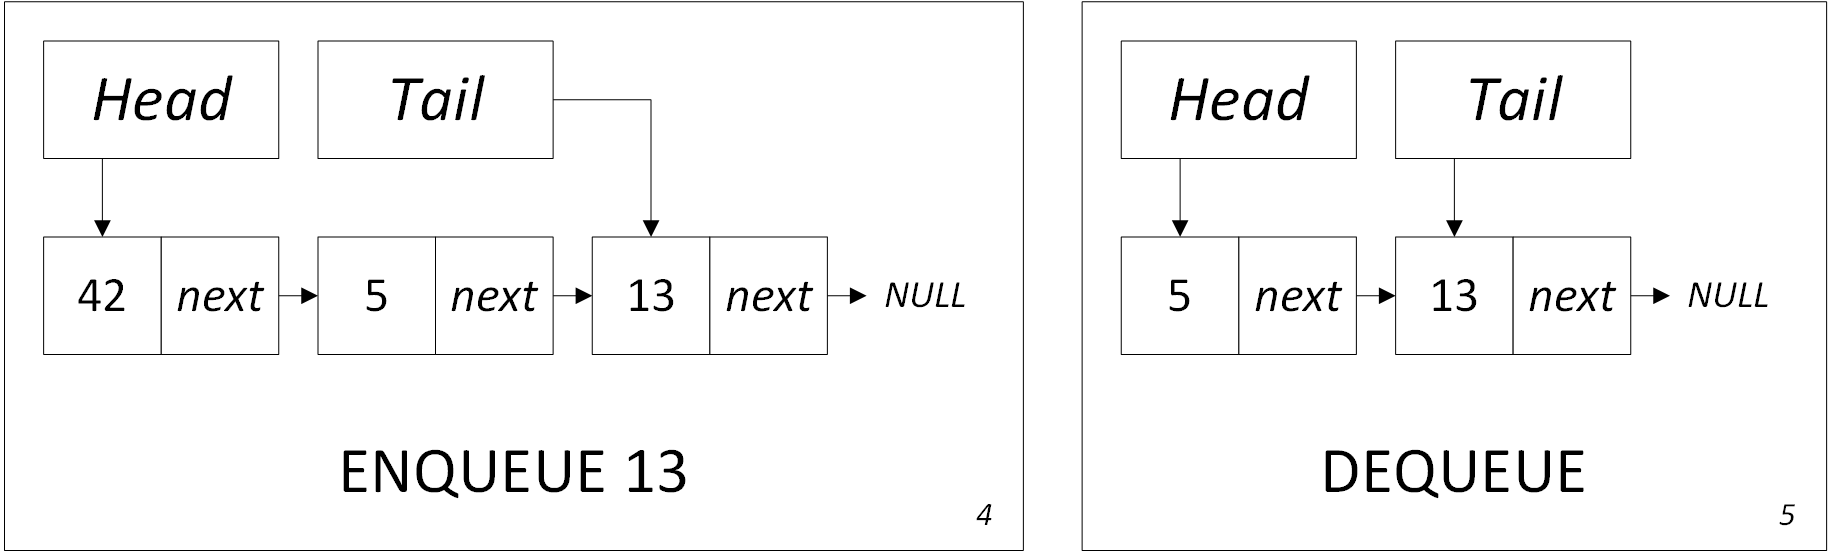
\includegraphics[scale=0.60]{img/files/Files_4_Liste_Chainee_Usage_pack_2.png}
\end{center}

\smallskip

Les principales opérations se résument ainsi :

\begin{itemize}
\item \TTBF{CreerFile() : File}\\
      La fonction alloue en mémoire la structure générale de la file, et elle fixe les tête et queue de la file à \TTBF{NULL}
\item \TTBF{Enfiler(File, Elt) : booléen}\\
      La fonction alloue en mémoire un nouvel élément, elle met son pointeur \textit{next} à \TTBF{NULL}, puis, si la file est vide, elle met les pointeurs de tête et de queue sur le nouvel élément, sinon, elle met l'adresse du nouvel élément sur le pointeur \textit{next} de l'élément pointé par la queue, et elle met à jour le pointeur de queue sur le nouvel élément
\item \TTBF{Défiler(File) : booléen}\\
      La fonction retourne une erreur si la file est vide, sinon, elle récupère tout d'abord l'adresse de l'élément suivant celui en tête, puis, elle libère l'élément en tête, puis, elle met à jour le pointeur de tête de la file vers l'adresse de l'élément suivant. Si l'élément suivant est \TTBF{NULL}, elle met à jour le pointeur de queue également
\item \TTBF{Vider(File) : entier}\\
      La fonction défile successivement tous les éléments jusqu'à obtenir la tête à \TTBF{NULL} (ne pas oublier que l'opération qui défile met à jour la queue dans le cas \TTBF{NULL})
\item \TTBF{Tête(File) : [Type Elt]}\\
      La fonction renvoie le contenu de l'élément en tête de file (le prochain élément qui sera défilé), ou s'il n'y en a pas, elle lève une exception, ou renvoie un pointeur \TTBF{NULL}, ou écrit un message d'erreur sans rien faire
\item \TTBF{Queue(File) : [Type Elt]}\\
      La fonction renvoie le contenu de l'élément en queue de file (le dernier élément qui sera défilé), ou s'il n'y en a pas, elle lève une exception, ou renvoie un pointeur \TTBF{NULL}, ou écrit un message d'erreur sans rien faire
\item \TTBF{Supprimer(File)}\\
      La fonction supprime la structure générale de la file en mémoire, éventuellement en la vidant juste avant
\end{itemize}

\bigskip

\vfillFirst

\vfillLast


\begin{center}
\textit{Ce document et ses illustrations ont été réalisés par Fabrice BOISSIER en octobre 2022}
\end{center}

\end{document}
